% options:
% thesis=B bachelor's thesis
% thesis=M master's thesis
% czech thesis in Czech language
% slovak thesis in Slovak language
% english thesis in English language
% hidelinks remove colour boxes around hyperlinks

\documentclass[thesis=M,czech]{FITthesis}[2014/05/6]

\usepackage[utf8]{inputenc} % LaTeX source encoded as UTF-8

\usepackage{graphicx} %graphics files inclusion
% \usepackage{amsmath} %advanced maths
% \usepackage{amssymb} %additional math symbols

\usepackage{dirtree} %directory tree visualisation

%-----------------------------------------------------
\usepackage[T1]{fontenc}
\usepackage{xcolor}
\usepackage{enumitem}
\usepackage{lipsum}




\usepackage{listings}
\usepackage{color}

\definecolor{mygreen}{rgb}{0,0.6,0}
\definecolor{mygray}{rgb}{0.5,0.5,0.5}
\definecolor{mymauve}{rgb}{0.58,0,0.82}


\lstset{ %
  backgroundcolor=\color{white},   % choose the background color; you must add \usepackage{color} or \usepackage{xcolor}
  basicstyle=\footnotesize,        % the size of the fonts that are used for the code
  breakatwhitespace=false,         % sets if automatic breaks should only happen at whitespace
  breaklines=true,                 % sets automatic line breaking
  captionpos=b,                    % sets the caption-position to bottom
  commentstyle=\color{mygreen},    % comment style
  deletekeywords={...},            % if you want to delete keywords from the given language
  escapeinside={\%*}{*)},          % if you want to add LaTeX within your code
  extendedchars=true,              % lets you use non-ASCII characters; for 8-bits encodings only, does not work with UTF-8
  frame=single,                    % adds a frame around the code
  keepspaces=false,                 % keeps spaces in text, useful for keeping indentation of code (possibly needs columns=flexible)
  keywordstyle=\color{blue},       % keyword style
  language=Java,                 % the language of the code
  morekeywords={*,...},            % if you want to add more keywords to the set
  numbers=left,                    % where to put the line-numbers; possible values are (none, left, right)
  numbersep=5pt,                   % how far the line-numbers are from the code
  numberstyle=\tiny\color{mygray}, % the style that is used for the line-numbers
  rulecolor=\color{black},         % if not set, the frame-color may be changed on line-breaks within not-black text (e.g. comments (green here))
  showspaces=false,                % show spaces everywhere adding particular underscores; it overrides 'showstringspaces'
  showstringspaces=false,          % underline spaces within strings only
  showtabs=false,                  % show tabs within strings adding particular underscores
  stepnumber=2,                    % the step between two line-numbers. If it's 1, each line will be numbered
  stringstyle=\color{mymauve},     % string literal style
  tabsize=2,                       % sets default tabsize to 2 spaces
  title=\lstname                   % show the filename of files included with \lstinputlisting; also try caption instead of title
}

\renewcommand{\lstlistingname}{Ukázka zdroj. kódu}% Listing -> Algorithm
\renewcommand{\lstlistlistingname}{Seznam ukázek zdroj. kódu}

% --------------------------------------------------------------------

% % list of acronyms
% \usepackage[acronym,nonumberlist,toc,numberedsection=autolabel]{glossaries}
% \iflanguage{czech}{\renewcommand*{\acronymname}{Seznam pou{\v z}it{\' y}ch zkratek}}{}
% \makeglossaries

\newcommand{\tg}{\mathop{\mathrm{tg}}} %cesky tangens
\newcommand{\cotg}{\mathop{\mathrm{cotg}}} %cesky cotangens

% % % % % % % % % % % % % % % % % % % % % % % % % % % % % % 
% ODTUD DAL VSE ZMENTE
% % % % % % % % % % % % % % % % % % % % % % % % % % % % % % 

\department{Katedra softwarového inženýrství}
\title{WebGephi - Webové rozhraní pro Gephi}
\authorGN{Václav} %(křestní) jméno (jména) autora
\authorFN{Čokrt} %příjmení autora
\authorWithDegrees{Bc. Václav Čokrt} %jméno autora včetně současných
% akademických titulů
\supervisor{Ing. Jaroslav Kuchař}
\acknowledgements{Děkuji Ing. Jaroslavu Kuchařovi za možnost pracovat na zajímavém tématu, své přítelkyni za podporu a trpělivost během mé studijní vytíženosti a v neposlední řadě samozřejmě
své rodině za podporu při studiu.}
\abstractCS{Cílem této práce je vytvoření webové aplikace \textit{WebGephi}, která zpřístupní funkcionalitu aplikace 
\textit{Gephi}\footnote{\textit{Gephi}\cite{gephi} je opensource desktopová aplikace sloužící k vizualizaci a manipulaci s grafy.} pomocí RESTful webových služeb. 

První část práce je zaměřena na analýzu aplikace \textit{Gephi} a specifikaci požadavků nové aplikace. Na základě těchto požadavků je navrhnuta architektura aplikace
a struktura REST rozhraní. Protože aplikace bude sloužit především jako poskytovatel služeb jiným aplikacím, práce se podrobně zabývá i možnými způsoby autorizace a autentizace.
Závěrečná část práce se zabývá samotnou implementací \textit{WebGephi}.

Součástí řešení je i implementace ukázkové klientská aplikace - grafické nadstavby - demonstrující funkcionalitu \textit{WebGephi}.}

\abstractEN{The aim of this thesis is to create the \textit{WebGephi} application that exposes the 
\textit{Gephi}\footnote{\textit{Gephi}\cite{gephi} is an open source desktop application for graphs visualization and manipulation.} 
application functionality as a RESTful web service. 

The first part is focused on \textit{Gephi} analysis and requirements specification of the new application. Based on these requirements, application architecture 
and structure of the REST interface is designed. Because the main purpose of \textit{WebGephi} is to provide services to other applications, 
this thesis focuses on possible ways of authorization and authentication too. The final part discusses the \textit{WebGephi} implementation.

Part of the solution will also be a sample client 
application - graphical interface - which demonstrates the \textit{WebGephi} functionality.}
\placeForDeclarationOfAuthenticity{V~Praze}
\declarationOfAuthenticityOption{4} %volba Prohlášení (číslo 1-6)
\keywordsCS{Gephi, Gephi Toolkit, graf, REST, RESTful, webové služby, webová aplikace}
\keywordsEN{Gephi, Gephi Toolkit, graph, REST, RESTful, web services, web application}
\newtheorem{definice}{Definice}

%\makeatletter
%\let\@makechapterheadOLD\@makechapterhead
%\renewcommand{\@makechapterhead}{\mbox{}\vspace*{-30pt}\@makechapterheadOLD}
%\let\@makeschapterheadOLD\@makeschapterhead
%\renewcommand{\@makeschapterhead}{\mbox{}\vspace*{-30pt}\@makeschapterheadOLD}
%\makeatother

\begin{document}

\begin{introduction}
	\uv{Graf je základním objektem teorie grafů. Jedná se o reprezentaci množiny objektů, u které chceme znázornit, 
	že některé prvky jsou propojeny. Objektům se přiřadí vrcholy a jejich propojení značí hrany mezi nimi. 
	Grafy slouží jako abstrakce mnoha různých problémů. Často se jedná o zjednodušený model nějaké skutečné 
	sítě (například dopravní), který zdůrazňuje topologické vlastnosti objektů (vrcholů) a zanedbává geometrické vlastnosti, například přesnou polohu.\cite{wiki:graf}}
		
	Graf tedy můžeme chápat jako zjednodušený obraz nějaké skutečnosti -
	seznam lidí a vztahů mezi nimi, množina webových stránek a hypertextových odkazů, cokoli, co lze znázornit jako množinu uzlů a hran (vztahů mezi nimi).
	
	Gephi\cite{gephi} je desktopová platforma sloužící k analýze grafů. Umožňuje interaktivně měnit rozložení grafů na základě jejich struktury, vypočítávat metriky (PageRank, shlukovací koeficient, \ldots), 
	filtrovat uzly podle jejich vlastností a mnoho dalšího. To vše slouží k tomu, aby uživatel byl schopný v grafu najít skryté závislosti a mohl lépe pochopit (a vizualizovat) strukturu grafu.
	
	Jednou z hlavních výhod \textit{Gephi} je jeho rozšiřitelnost. Kdokoli může vytvořit svou vlastní funkci k manipulaci s grafem a ve formě pluginu ji přidat do aplikace.
	
	Aplikace \textit{WebGephi} by měla zachovat tyto vlastnosti a navíc přidat výhody plynoucí ze standardizovaného rozhraní webové aplikace.  
\end{introduction}

\chapter{Cíl práce}
Cílem této práce je vytvořit webovou aplikaci poskytující funkcionalitu \textit{Gephi}. Hlavní rozhraní této aplikace bude založeno na architektuře REST.


\textit{\uv{
REST (Representational State Transfer) – je architektura rozhraní, navržená pro distribuované prostředí. REST navrhnul a popsal v roce 2000 Roy 
Fielding (jeden ze spoluautorů protokolu http) v rámci disertační práce Architectural Styles and the Design of Network-based Software Architectures. 
V kontextu práce je nejzajímavější kapitola 5, ve které Fielding odvozuje principy RESTu na základě známých přístupů k architektuře. 
Rozhraní REST je použitelné pro jednotný a snadný přístup ke zdrojům (resources). Zdrojem mohou být data, stejně jako stavy aplikace 
(pokud je lze popsat konkrétními daty). REST je tedy na rozdíl od známějších XML-RPC či SOAP, orientován datově, nikoli procedurálně. 
Všechny zdroje mají vlastní identifikátor URI a REST definuje čtyři základní metody pro přístup k nim.}}\cite{wiki:rest}

\textit{WebGephi} bude sloužit jen jako poskytovatel služeb pro jiné (klientské) aplikace. Tyto aplikace budou pomocí webových služeb přistupovat k \textit{WebGephi} (nahrávat grafy, aplikovat na ně funkce, exportovat výsledky, \ldots)
a komunikovat s koncovým uživatelem přes vlastní grafické rozhraní. Klientské aplikace mohou být webové, desktopové i mobilní aplikace. Přístup klientských aplikací samozřejmě bude také třeba řídit. 
\textit{WebGephi} tedy kromě REST rozhraní bude poskytovat také grafické rozhraní pro registraci a správu uživatelů a klientských aplikací.

Hlavní výhody \textit{WebGephi} budou jednoduché, standardizované, deklarativní rozhraní. \textit{Gephi} sice poskytuje knihovnu pro práci s grafy, \textit{Gephi Toolkit}\cite{gephi:toolkit}, ta je však dosti složitá na použití. 
Klientské aplikace budou moci jednoduše přistupovat k tomuto rozhraní pomocí HTTP protokolu, na kterém je v naprosté většině založena REST architektura. To umožní jak
jednoduché prozkoumávání rozhraní (např. pomocí webového prohlížeče), tak strojové zpracování koncovými klientskými aplikacemi.

Pro koncového uživatele je hlavní výhodou možnost použití bez nutnosti instalace (ve spolupráci s klientskými aplikacemi), použití jako centrálního úložiště grafů a možnost sdílení s jinými uživateli.

\textit{WebGephi} bude postaveno nad již zmíněnou knihovnou \textit{Gephi Toolkit}. Ta obsahuje základní moduly \textit{Gephi} (bez GUI\footnote{Graphical User Interface - grafické uživatelské rozhraní} funkcionality) ve formě jednoduché Java knihovny.
V prvním kroku bude třeba určit, jaká funkcionalita bude implementována ve \textit{WebGephi}. Následně bude třeba analyzovat strukturu knihovnu \textit{Gephi Toolkit} a s její pomocí tuto funkcionalitu implementovat.
Dále bude potřeba navrhnout a implementovat strukturu REST rozhraní a způsob autentizace uživatelů.

Součástí práce je i implementace ukázkové klientské aplikace. Ta bude využívat naprostou většinu funkcionality WebGephi a demonstrovat její funkčnost.


\chapter{Analýza}
Cílem této kapitoly je hlubší náhled do problematiky a analýza dostupných nástrojů. Na konci kapitoly bychom měli mít jasno v tom, zda a jak je tento úkol řešitelný.

Nejdříve si představíme aplikaci \textit{Gephi} a její možnosti. Určíme, jakou funkcionalitu bude možné a vhodné přenést do \textit{WebGephi}. Dále představíme strukturu knihovny \textit{Gephi Toolkit}
a nastíníme, zda a jakým způsobem bude možné požadovanou funkcionalitu implementovat. Aplikace bude také muset řešit autentizaci a autorizaci přístupu. V poslední části si tedy také představíme
standardní řešení tohoto problému.

\section{Gephi}
\textit{\uv{Gephi je platforma pro vizualizaci a prozkoumávání všech druhů sítí a
komplexních systémů, dynamických a hierarchických grafů. Je dostupný pro Windows, Linux a Mac OS x. \textit{Gephi} je open-source a zdarma.}}\footnote{Volný překlad z oficiálních stránek \textit{Gephi}\cite{gephi}. Orig.: \uv{Gephi is an interactive visualization and exploration platform for all kinds of networks and complex systems, dynamic and hierarchical graphs.
Runs on Windows, Linux and Mac OS X. \textit{Gephi} is open-source and free.}}

Jedná se tedy o volně dostupný, bezplatný nástroj pro práci s grafy. První veřejně dostupná verze měla číslo 0.6alpha1 a vyšla v roce 2008.
Původně se jednalo o studentskou práci francouzských studentů\footnote{The
University of Technology of Compiègne (Université de Technologie de Compiègne or
UTC)}. V současnosti se o jeho vývoj stará \uv{Gephi Consortium}\cite{gephi:consortium}.

Přesto, že i současná verze (0.8.2-beta) je stále betaverze, jedná se o široce
používaný software s rozsáhlou funkcionalitou. Budoucí verze číslo 0.9 by měla být výrazným krokem v evoluci \textit{Gephi}, bude obsahovat změny v samotném jádru aplikace.
Jedná se o velmi živý projekt, který je v neustálém vývoji.

\textit{Gephi} je napsáno v programovacím jazyku Java. Je založeno na \textit{NetBeans}\footnote{https://\textit{NetBeans}.org/} platformě, grafické rozhraní využívá framework Swing.  

\subsection{Struktura aplikace}
Zde si představíme strukturu aplikace \textit{Gephi} a její uživatelské rozhraní.

Základní jednotkou při práci s \textit{Gephi} je \uv{Projekt}. Aplikace může pracovat vždy jen s jedním projektem. Projekt je nejvyšší jednotkou v \textit{Gephi}, může být ukládán a 
načítán z disku a může obsahovat jeden nebo více \uv{Pracovních prostorů} (Workspace). V aplikaci je vždy aktivní jen jeden Workspace. Workspace představuje 
pracovní plochu, na které se mohou vytvářet a editovat grafy.
 
Uživatelské rozhraní se skládá ze tří záložek - Přehled, Laboratoř dat a Náhled.

\subsubsection{Záložka Přehled}
Jedná se o nejdůležitější záložku (obr. \ref{fig:gephi-overview}). Na středu je vidět náhled grafu a po stranách jsou dostupné funkce, které lze na graf aplikovat. Po
aplikaci funkce je graf okamžitě překreslen. S grafem lze manipulovat i ručně pomocí nástrojů na svislé liště na levé straně náhledu grafu.

\begin{figure}\centering
 	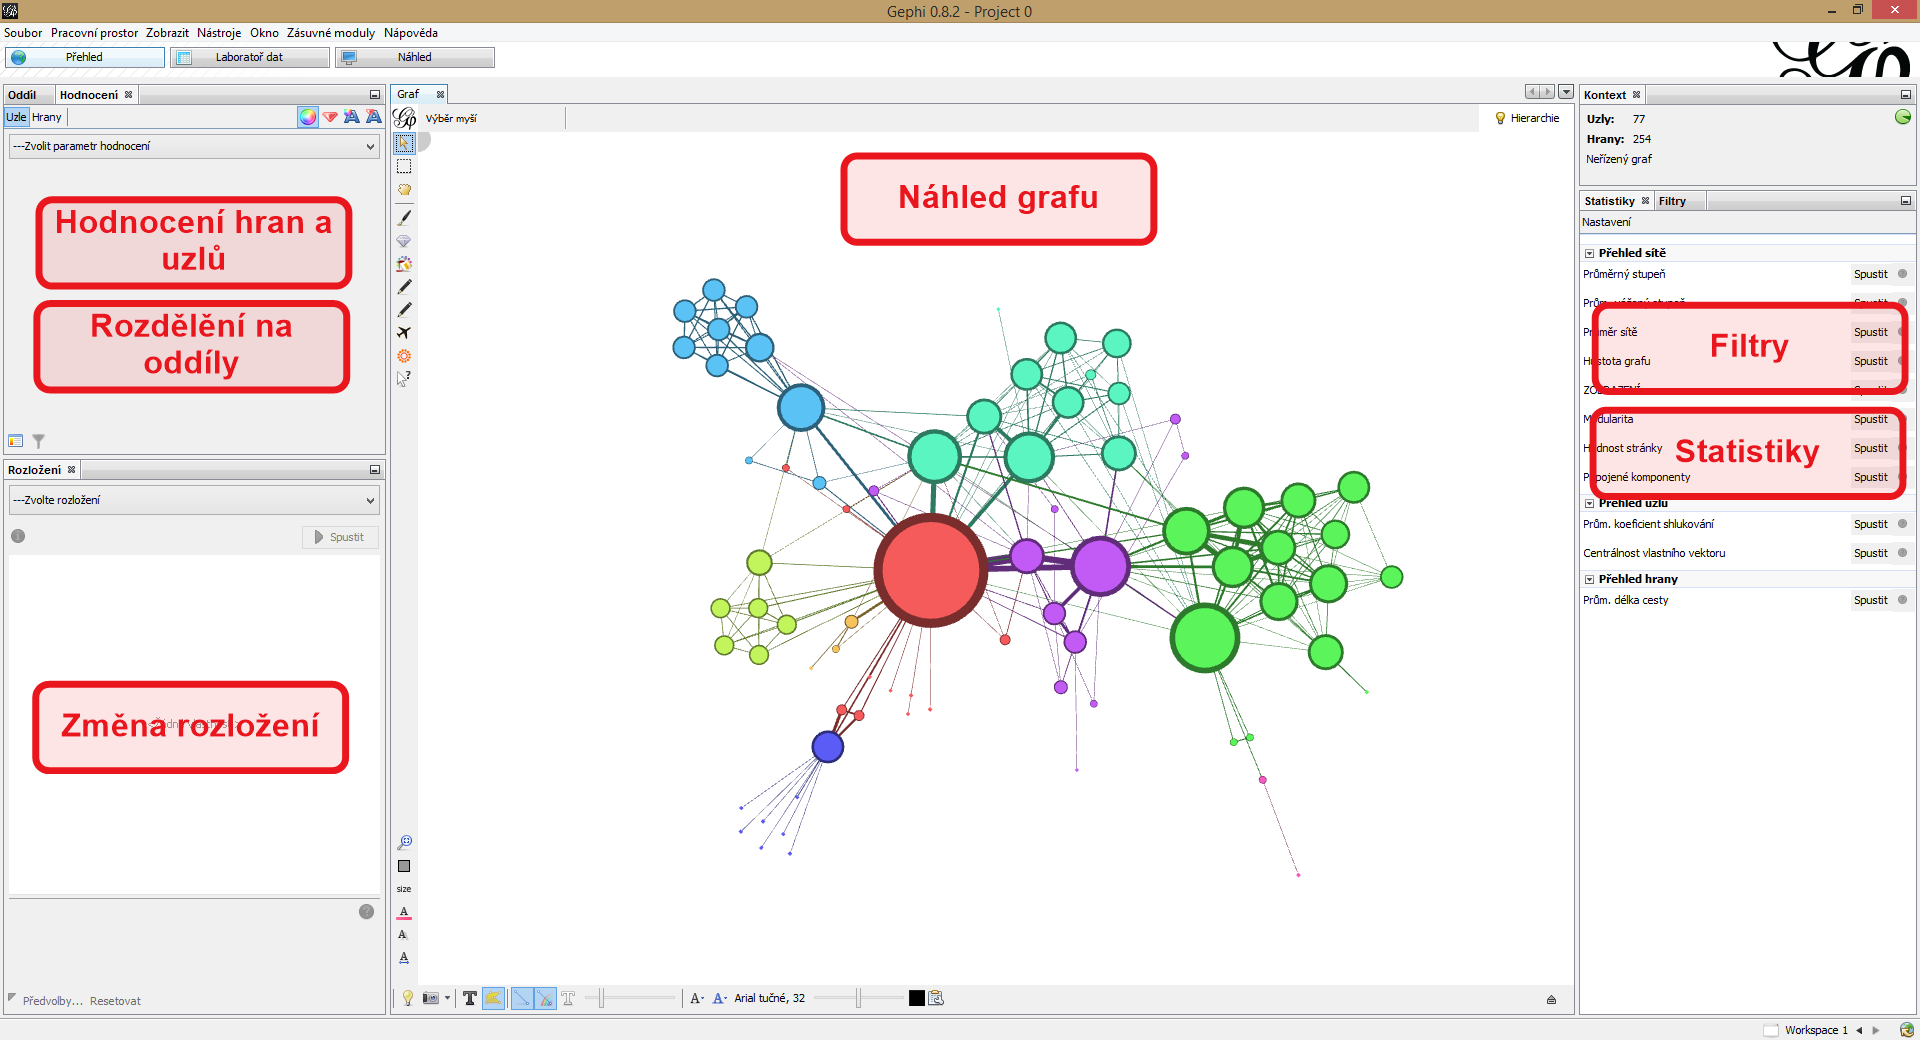
\includegraphics[width=1\textwidth]{images/gephi/gephi_overview_final}
 	\caption[Záložka \uv{Přehled}]{Záložka \uv{Přehled}}\label{fig:gephi-overview}
\end{figure}

\subsubsection{Záložka Laboratoř dat}
Tato záložka (obr. \ref{fig:gephi-lab}) slouží k úpravě zdrojových dat grafu. Uzly a hrany lze vkládat ručně nebo importovat z různých zdrojů (soubor, databáze, \ldots). Na středu je vidět
seznam uzlů a hran aktuálního grafu. S daty lze provádět po sloupcích (atributech) i hromadné operace.

\begin{figure}\centering
 	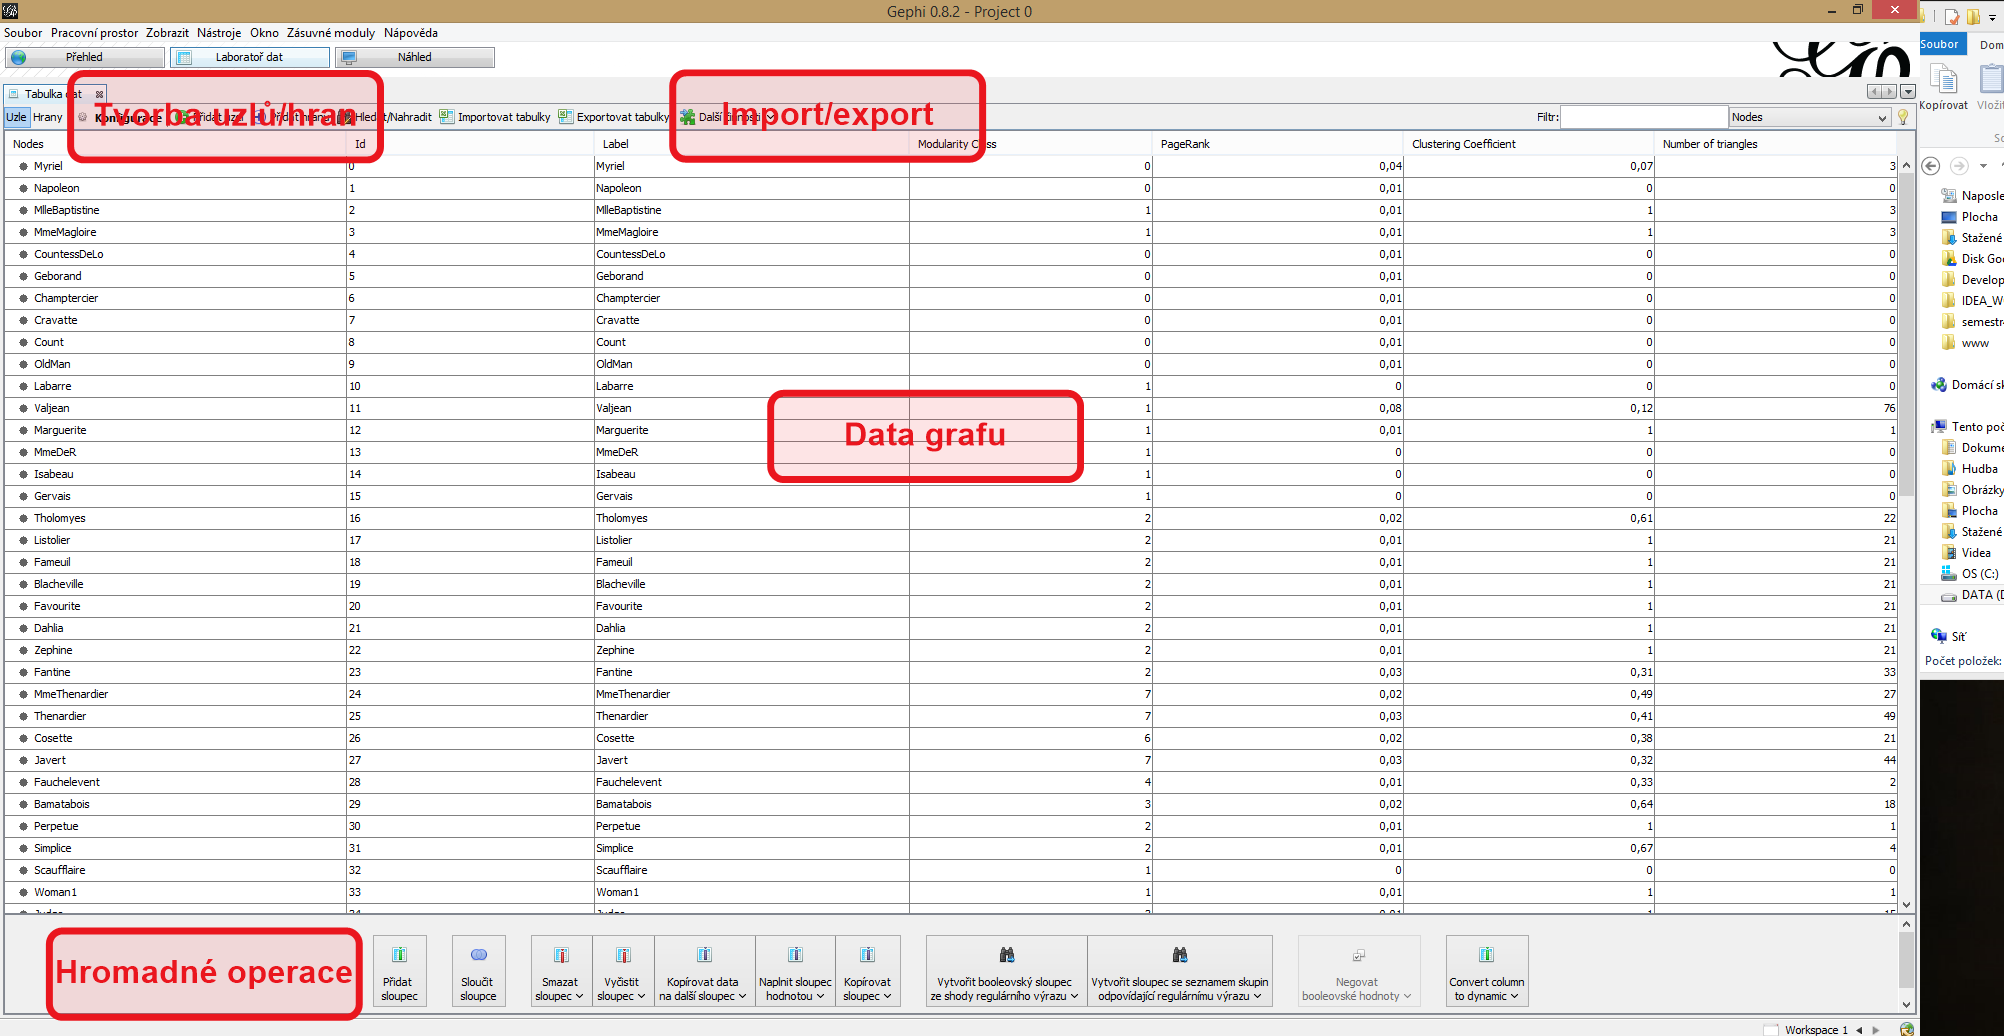
\includegraphics[width=1\textwidth]{images/gephi/gephi_lab_final}
 	\caption[Záložka \uv{Laboratoř dat}]{Záložka \uv{Laboratoř dat}}\label{fig:gephi-lab}
\end{figure}

\subsubsection{Záložka Náhled}
Poslední záložka (obr. \ref{fig:gephi-exp}) slouží k vizuální úpravě grafu. Typicky se používá před exportem výsledku do obrázku. Lze nastavovat velikost hran, uzlů, nastavení popisků, průhlednost, \ldots
Výsledný graf lze exportovat ve formátu png, svg a pdf.

\begin{figure}\centering
 	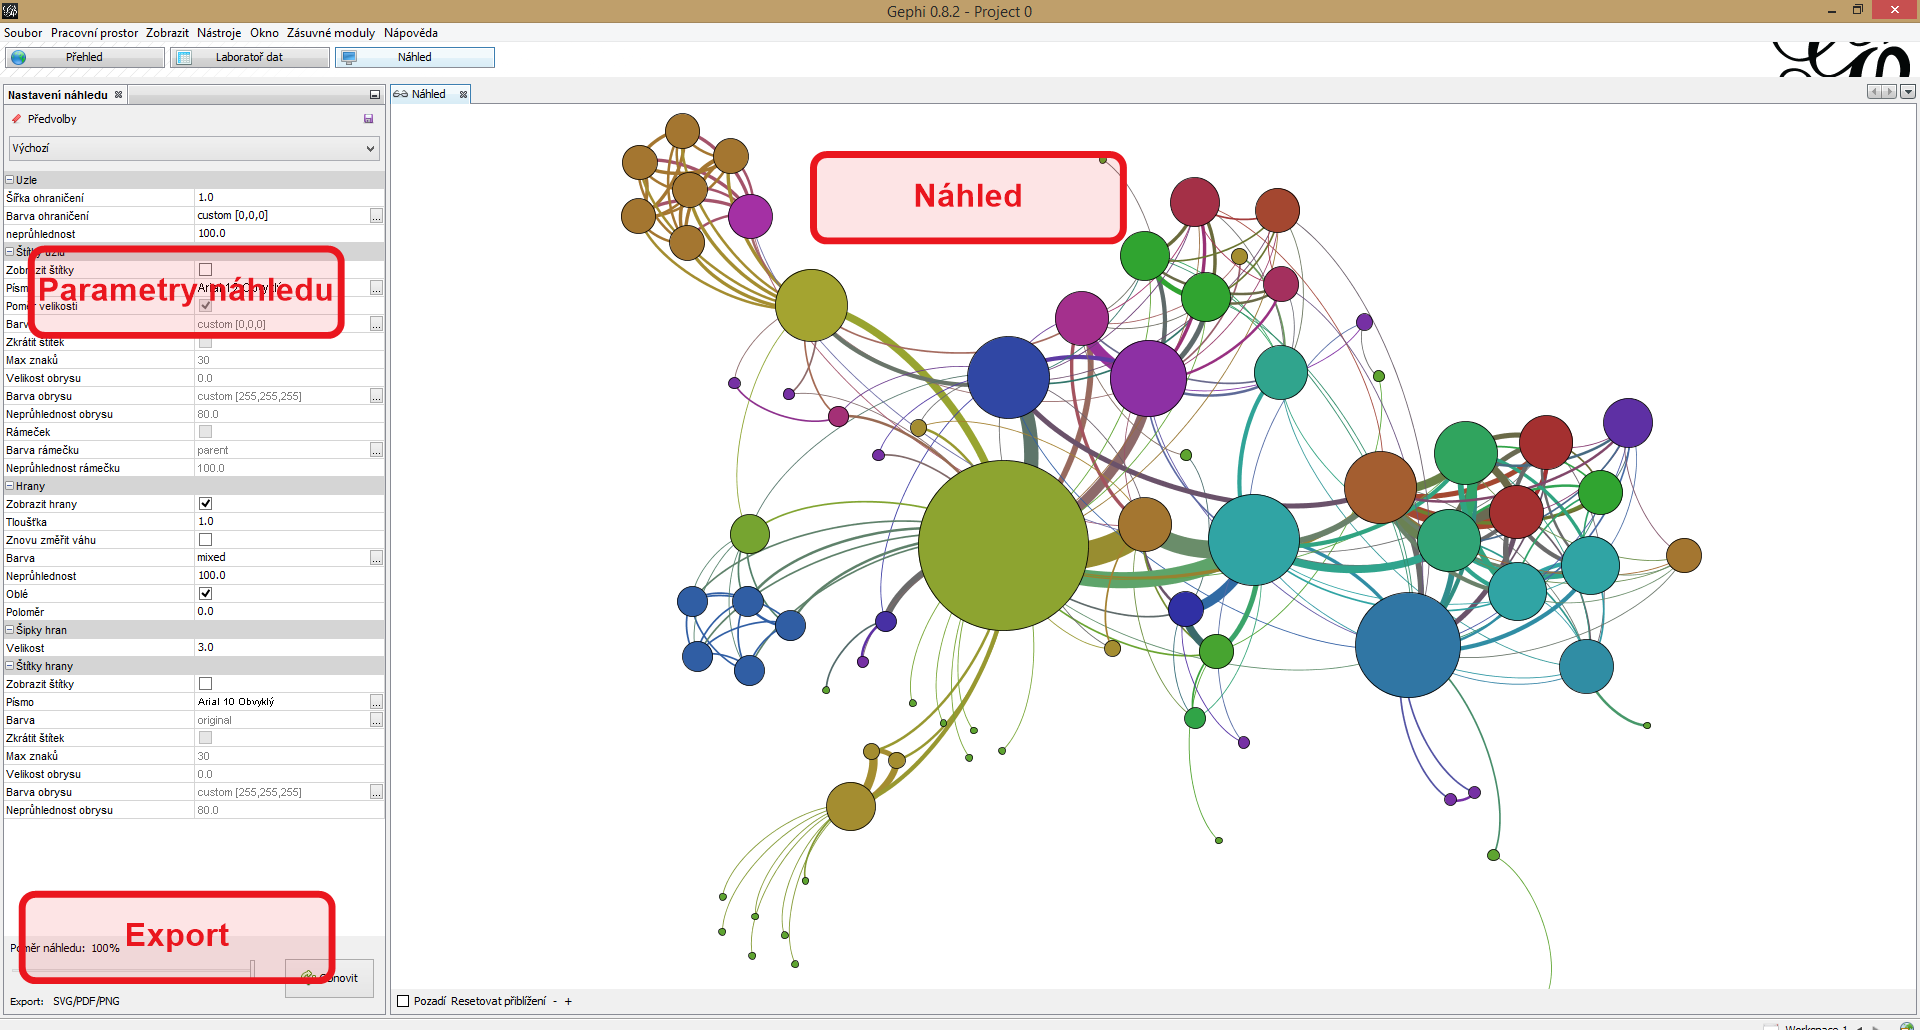
\includegraphics[width=1\textwidth]{images/gephi/gephi_exp_final}
 	\caption[Záložka \uv{Náhled}]{Záložka \uv{Náhled}}\label{fig:gephi-exp}
\end{figure}

\subsection{Funkcionalita}
Zde podrobně popíšeme funkcionalitu \textit{Gephi}.

\subsubsection{Import a export}
\textit{Gephi} ukládá projekty do svého interního formátu \texttt{gephi}. Ten kromě samotného grafu ukládá i strukturu projektu a jeho nastavení. Pro výměnu dat mezi
aplikacemi jsou důležitější standardizované formáty. \textit{Gephi} umí načítat téměř jakýkoli formát vhodný pro ukládání grafu, včetně \texttt{csv}, \texttt{graphML} a
\texttt{gexf}. Do těchto formátů umí samozřejmě grafy i exportovat.

Nejvhodnější z těchto formátů je jednoznačně formát \texttt{gexf}\cite{gexf}. Ten je schopen uložit všechny důležité informace včetně hierarchických a dynamických grafů a je
prakticky standardem to tomto oboru. Jedná se o xml formát s relativně jednoduchou strukturou\footnote{Přesná struktura je definována standardně pomocí xml schématu: http://www.gexf.net/1.2draft/gexf.xsd}. Základem je seznam uzlů a hran (včetně jejich atributů).

V příloze \ref{fig:gephi-formats-comparation} můžete vidět porovnání dostupných formátů.

\textit{Gephi} je schopno načítat grafy také SQL databáze (stačí specifikovat potřebný SQL dotaz). 

Kromě datového exportu je dostupný taká export vizuální reprezentace grafu. Dostupné jsou formáty \texttt{pdf}, \texttt{svg} a \texttt{png}.

\subsubsection{Grafové funkce}
Hlavní silou \textit{Gephi} je manipulace s grafem jako s celkem. \textit{Gephi} už v základu obsahuje množství takovýchto funkcí a je možné je dále rozšířit pomocí pluginů.
Funkce jsou podle zaměření rozděleny do několika skupin.

\paragraph{Rozložení}
Funkce pro změnu rozložení slouží k systematickému přeskupení uzlů. Může se jednat o velmi jednoduché funkce, např. \texttt{Otočení podle směru hodinových ručiček}, která jen otočí graf o
definovaný úhel, ale i o velmi specifikované funkce, jako je \texttt{Force Atlas}, který přeskupuje uzly podle jejich vazeb k okolí. Obecně se jedná o jakékoli funkce,
které mění poziční atributy uzlů.

Některé funkce podporují interaktivní režim, kdy se funkce spustí v nekonečné smyčce, takže okamžitě vidíme, jaký vliv na rozložení grafu má změna atributů. Když jsme s rozložením spokojeni,
stačí funkci zastavit. Ukázku změny rozložení můžete vidět na obr. \ref{fig:gephi-layout}.

\begin{figure}\centering
 	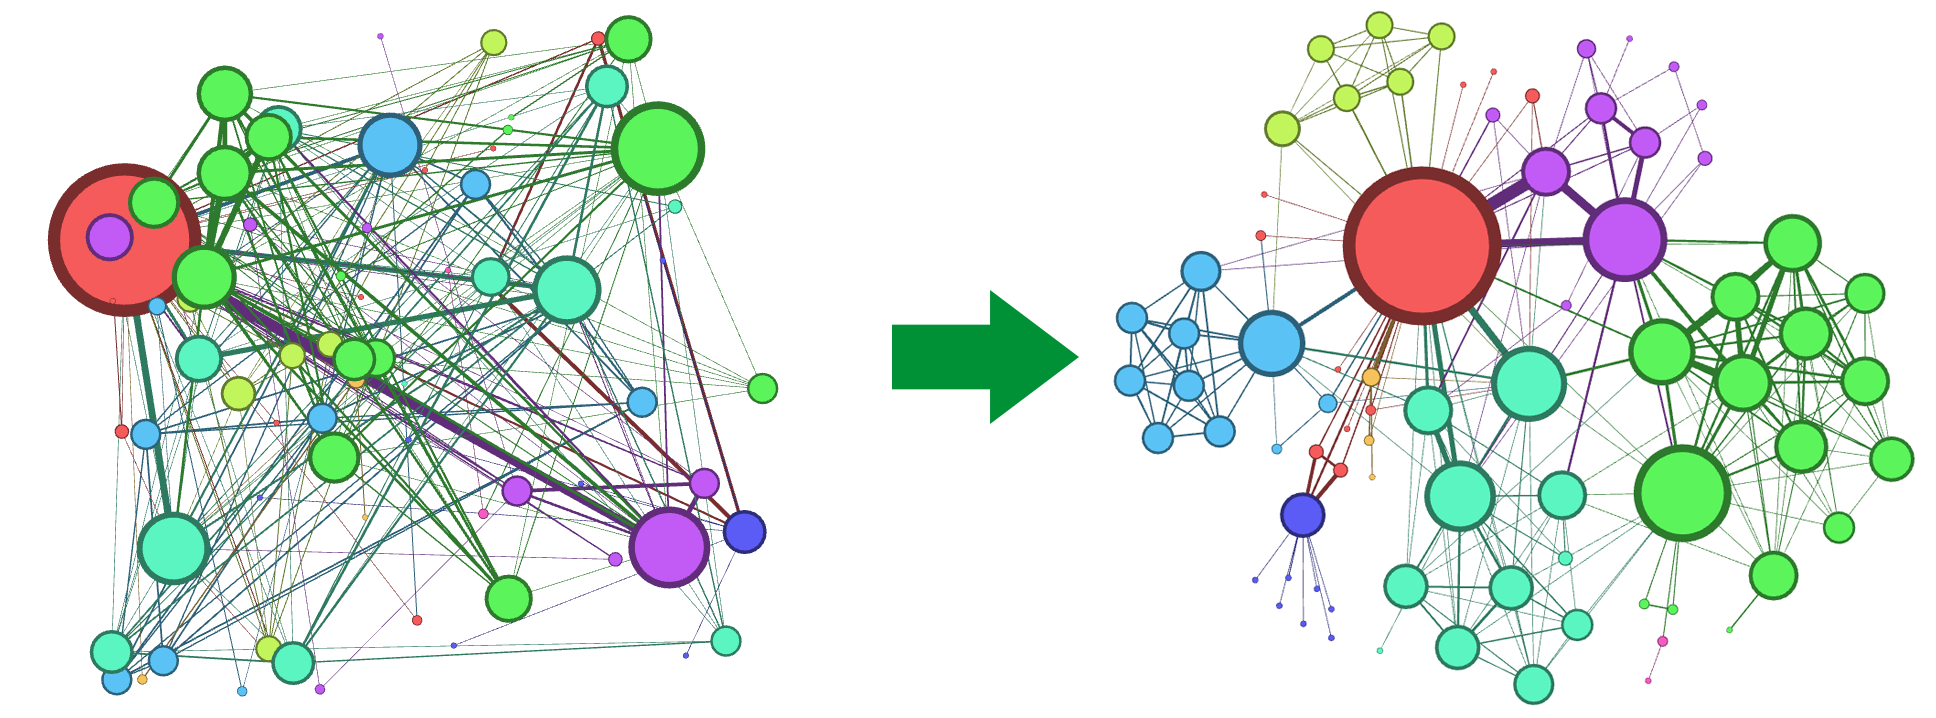
\includegraphics[width=1\textwidth]{images/gephi/layout_before-after}
 	\caption[Změna rozložení podle funkce \texttt{Foce Atlas 2}]{Změna rozložení podle funkce \texttt{Foce Atlas 2}.}\label{fig:gephi-layout}
\end{figure}

\paragraph{Statistiky a metriky}
Tako kategorie funkcí je určená k výpočtu metrik nad grafem. Výstupem funkce je přidání jednoho nebo více atributů k uzlům nebo hranám. Navíc je zobrazena
shrnující zpráva (obr. \ref{fig:gephi-pagerank}), která typicky prezentuje rozložení hodnot atributů v grafu. Jako příklad statistické funkce lze uvést např. \texttt{Hodnost stránky} (PageRank\footnote{Algoritmus
pro ohodnocení důležitosti webových stránek na základě struktury hypertextových odkazů.}).

\begin{figure}\centering
 	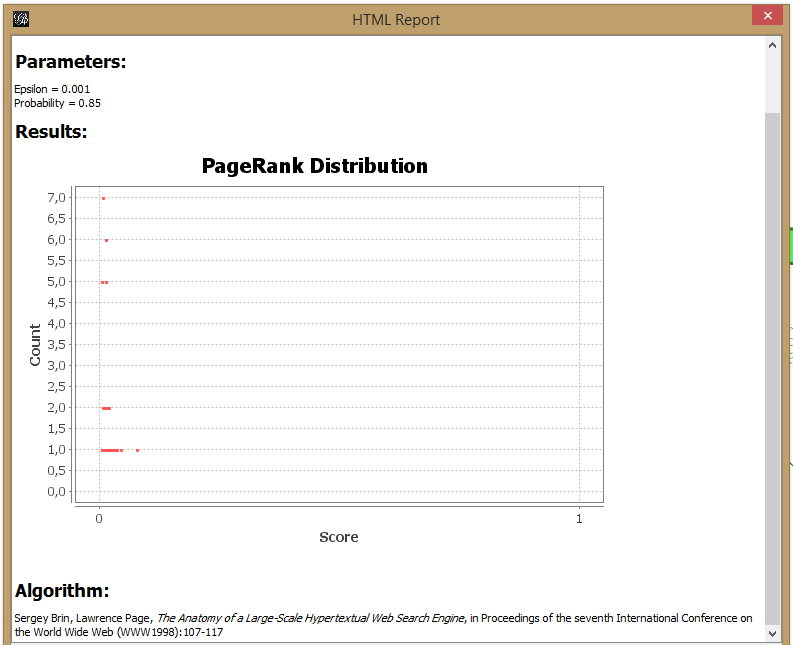
\includegraphics[width=0.5\textwidth]{images/gephi/statistics-pagerank}
 	\caption[Report po aplikaci funkce \texttt{PageRank}]{Report po aplikaci funkce \texttt{PageRank}PageRank}\label{fig:gephi-pagerank}
\end{figure}

\paragraph{Hodnocení}
Hodnocení slouží k lepší vizuální reprezentaci hodnot atributů (vypočtených např. pomocí již zmíněných statistických funkcí). Podle hodnoty atributu lze 
měnit barvu nebo velikost uzlů a hran. Aplikaci \uv{hodnocení} můžeme vidět na obr. \ref{fig:gephi-ranking}.

\begin{figure}\centering
 	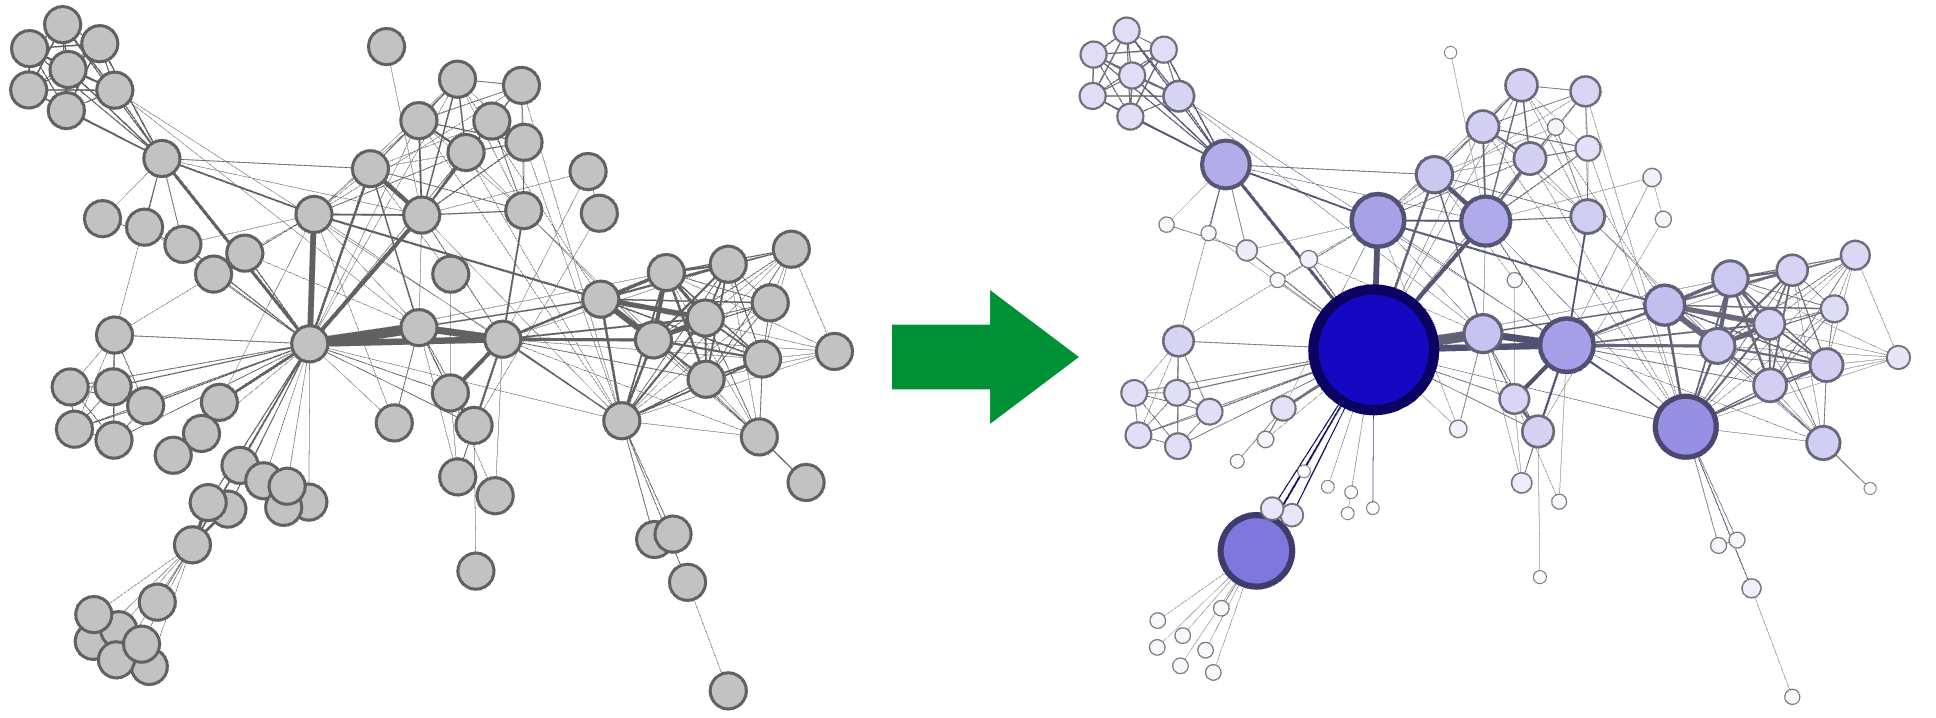
\includegraphics[width=1\textwidth]{images/gephi/ranking_before-after}
 	\caption[Hodnocení barvou a velikostí podle funkce \texttt{PageRank}]{Hodnocení barvou a velikostí podle funkce \texttt{PageRank}.}\label{fig:gephi-ranking}
\end{figure}

\paragraph{Rozdělení na oddíly}
Rozdělení na oddíly má podobnou funkci jako \uv{hodnocení}. V tomto případě se obarvují uzly se stejnou hodnotou atributu na stejnou barvu (lze použít jen na celočíselné
atributy). Tyto uzly lze také seskupit do jednoho uzlu, jehož velikost je závislá na počtu uzlů, které obsahuje. Ukázku můžete vidět na obr. \ref{fig:gephi-grouping}.

\begin{figure}\centering
 	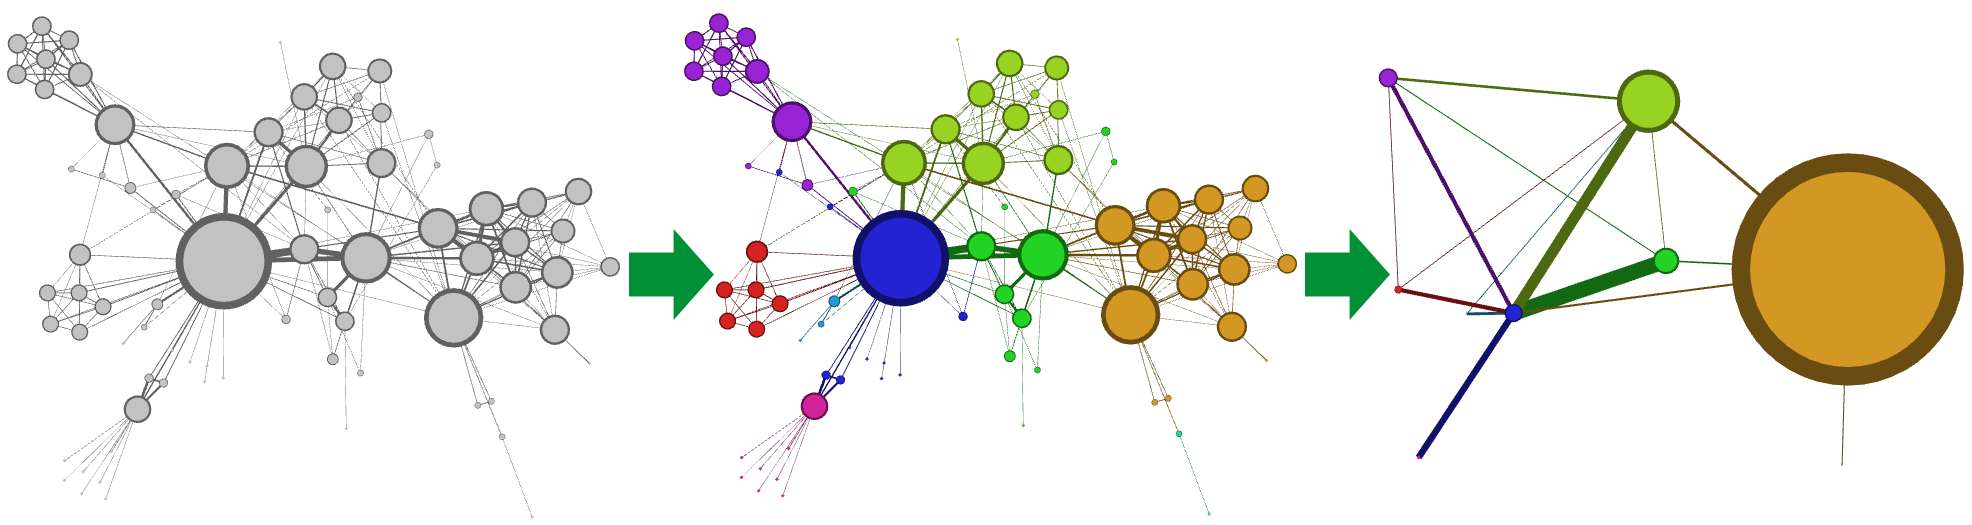
\includegraphics[width=1\textwidth]{images/gephi/grouping_before-after}
 	\caption[Rozdělení na oddíly podle hodnoty atributu \texttt{Modularity Class}]{Rozdělení na oddíly podle hodnoty atributu \texttt{Modularity Class}.}\label{fig:gephi-grouping}
\end{figure}

\paragraph{Filtry}
Ve velkých grafech je pro uživatele těžké se orientovat, je zahlcen velkým množstvím uzlů a hran. Pro tento účel obsahuje \textit{Gephi} filtry. Na základě nejrůznějších podmínek, většinou 
závislých na hodnotě atributů, lze uzly filtrovat (odstranit) z grafu. Jednoduché filtry lze navíc řetězit pomocí logických operátorů do složitějších výrazů.

Příklad aplikace jednoduchého filtru můžete vidět na obr. \ref{fig:gephi-filter}.

\begin{figure}\centering
 	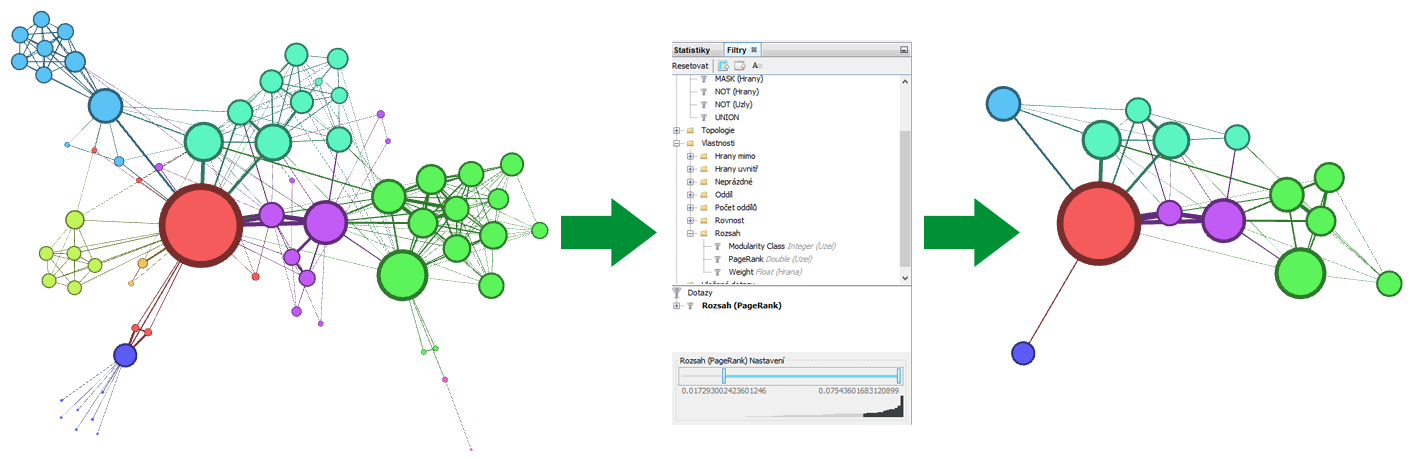
\includegraphics[width=1\textwidth]{images/gephi/filter_before-after}
 	\caption[Aplikace filtru \texttt{Rozsah} na základě hodnoty funkce \texttt{PageRank}]{Aplikace filtru \texttt{Rozsah} na základě hodnoty funkce \texttt{PageRank}.}\label{fig:gephi-filter}
\end{figure}

\paragraph{Generování grafu}
Pokud nemáme žádný vhodný graf (např. pro testování vyvíjeného pluginu), \textit{Gephi} poskytuje možnost vygenerování grafu. V základu je možnost generování jen náhodného grafu, kde můžeme
nastavit pouze požadovaný počet hran a uzlů. Existují však pluginy, které možnosti \textit{Gephi} v tomto směru dále rozšiřují.

\subsubsection{Dynamické grafy}
\textit{Gephi} podporuje také dynamické grafy. Jedná se o běžný graf, kde každý uzel a hrana má nastavený interval platnosti. Většinou se jedná o časový rozsah.
Tímto způsobem lze zachytit vývoj skutečnosti, kterou graf představuje, v čase.

\textit{Gephi}, kromě běžných operací, umí pomocí časové osy takovýto graf přehrát. Jedná se vlastně o specifický filtr na základě hodnoty intervalu.

\subsubsection{Manuální editace}
\textit{Gephi} poskytuje také možnosti manuální editace, a to jak grafického znázornění grafu, tak datového modelu. V okně \uv{Graf} je v levém svislém panelu množství funkcí, které 
umožňují ruční, interaktivní editaci grafu - změnu velikosti uzlu, barvy, pozice, popisku, \ldots V \uv{Laboratoři dat} je zase kromě importu a exportu také možné ručně přidávat a odebírat
uzly a hrany, nastavovat ručně hodnoty atributů a popisků.

\subsubsection{Instalace pluginů}\label{part:instalace-pluginu}
Jak už bylo několikrát zmíněno, \textit{Gephi} poskytuje možnost snadného rozšíření funkcionality pomocí pluginů. Využívá přitom možností platformy \textit{NetBeans},
která je od základu přizpůsobena modulární architektuře. \textit{Gephi} plugin je \textit{NetBeans} plugin\footnote{Jedná se o zip archive obsahující deskriptor modulu a jednu 
nebo více Java knihoven, které implementují vlastní funkcionalitu.} využívající API \textit{Gephi}. \textit{Gephi} při startu automaticky načte všechny pluginy a tím rozšíří 
svou funkcionalitu. Využívá k tomu \textit{NetBeans} specifické řešení, tzv. \textit{Lookup API}\footnote{API pro volnou vazbu mezi moduly (pluginy). 
Modul deklaruje veřejné rozhraní SPI (\textit{Service Provider Interface}). Jiné pluginy pak mohou toto rozhraní implementovat
a deklarovat jako \textit{Service Provider} a tím rozšířit funkcionalitu. Implementace \textit{Lookup API} poté dokáže tyto implementace nalézt i během runtime a použít.}.  
Přesný způsob implementace není pro tuto práci podstatný, stačí vědět, že pouhou implementací nějakého rozhraní lze rozšířit funkcionalitu \textit{Gephi}. 
 
\section{Komponenty relevantní pro WebGephi}
\textit{Gephi} poskytuje opravdu rozsáhlé možnosti práce s grafy, od manuální editace až po aplikaci komplexních funkcí a práci s dynamickými grafy.
Ne všechna funkcionalita je však vhodná pro \textit{WebGephi}. Zde si určíme, jakou funkcionalitu je vhodné (a možné) implementovat ve \textit{WebGephi}.

\subsection{Cílový uživatel}
Nejdříve si musíme shrnout, jak vlastně bude vypadat cílový uživatel, k jakému účelu bude \textit{WebGephi} primárně používáno.

\subsubsection{Student, vývojář aplikací}
Jedním z typických uživatelů bude pravděpodobně student vysoké školy, který v rámci nějakého projektu (např. semestrální práce) bude 
mít za úkol analýzu grafu. Většinou to nebude jediný smysl aplikace, pouze jedna z jejích částí. Místo vlastní implementace pomocí \textit{Gephi Toolkit}
využije API \textit{WebGephi}. Nebude se tedy muset zabývat strukturou knihovny ani způsobem implementace. Navíc není omezen
cílovou platformou (např. není nucen psát aplikaci v jazyku Java).

Nemusí se samozřejmě jednat pouze o studenty. Stejně tak se může jednat o jakéhokoli vývojáře, který chce v rámci své aplikace
využít možností \textit{Gephi}. \textit{WebGephi} ho odstíní od detailů implementace \textit{Gephi Toolkit} a poskytne platformovou nezávislost.

\subsubsection{Tvůrce pluginů}
Dalším typickým uživatelem bude tvůrce algoritmů pro práci s grafy. \textit{Gephi} poskytuje možnost snadného rozšíření pomocí pluginů.
Pokud někdo takovýto plugin vytvoří, pomocí \textit{WebGephi} (a její klientské aplikace) může vytvořit demo pro prezentaci jeho funkcionality. Případní 
uživatelé pluginu tak nebudou nuceni instalovat plugin jen pro jeho vyzkoušení.

\subsection{Požadovaná funkcionalita WebGephi}
Je tedy vidět, že pro \textit{WebGephi} není nutné ani vhodné pokrýt celou funkcionalitu \textit{Gephi}.
\textit{WebGephi} bude zaměřeno na práci s již existujícími grafy, není nutné řešit manuální editaci grafu. Stejně tak není nutné
podporovat všechny formáty pro import a export. Naopak je nutné zachovat většinu grafových funkcí. Klíčovou
vlastností \textit{Gephi} je jeho rozšiřitelnost, je nezbytné aby \textit{WebGephi} tuto rozšiřitelnost zachovalo.

\subsubsection{Import a export}
Existuje mnoho různých formátů vhodných pro uložení grafu, včetně proprietárních formátů různých aplikací. \textit{Gephi} obsahuje podporu
pro většinu z nich. Aplikace\textit{WebGephi} bude podporovat import grafu ve stejném rozsahu jako \textit{Gephi}.
Základním formátem bude však formát \texttt{gexf}. Tento formát je ve svém oboru standard a z dostupných formátů
má největší možnosti (viz srovnání \ref{fig:gephi-formats-comparation}). Jedná se relativně jednoduchý formát založený na \texttt{xml}, je 
tedy snadno strojově zpracovatelný a díky definici ve formátu \texttt{xsd} je jednoznačný. 

Export grafu bude dostupný pouze ve formátu \textit{gexf}, který je nejkomplexnější a je schopen uchovat všechny potřebné informace.

Vizualizace grafu bude zodpovědností především klientských aplikací. Přesto je vhodné, aby i \textit{WebGephi} obsahovalo základní export v grafickém formátu.
Nejvhodnější z podporovaných formátů\footnote{\texttt{png}, \texttt{pdf} a \texttt{svg}} je \texttt{svg}. Jedná se o vektorový formát založený na \texttt{xml}, který je pro tento účel
vhodnější než rastrový formát \texttt{png}. A oproti \texttt{pdf} je možná jeho další editace. Formát \texttt{svg} je podporován většinou grafických editorů a všechny
hlavní webové prohlížeče obsahují nativní podporu pro jeho vizualizaci.

\subsubsection{Grafové funkce}
Grafové funkce budou nejdůležitější částí aplikace. WebGephi se nebude zabývat tvorbou grafu ve většině případů ani jeho vizualizací. Typické workflow 
bude \textit{načtení grafu} - \textit{aplikace funkcí} - \textit{export ve formátu gexf}.

Nejdůležitější bude podpora pro funkce \uv{Rozložení} a \uv{Statistiky}, které jsou nejpoužívanější. Pro lepší vizualizaci výsledků
je také potřeba podpora pro funkce \uv{Hodnocení}. \uv{Filtry} jsou zase nezbytnou funkcionalitou pro lepší orientaci v rozsáhlých grafech.
Podpora pro \uv{Generování grafů} a \uv{Rozdělení na oddíly} nemusí být součástí 
této práce, jedná se o méně využívané funkce. Struktura \textit{WebGephi} však musí umožnit snadné doplnění této funkcionality v budoucnu.

\section{Gephi Toolkit}
\textit{Gephi} je aplikace určená pro koncového uživatele. Kromě modulů obsahujících logiku pro práci s grafy obsahuje také moduly související s uživatelským
rozhraním, nápovědou\ldots Není tedy vhodné pro další použití v jiných aplikacích. Naštěstí \textit{Gephi} pro tyto účely poskytuje knihovnu \textit{Gephi Toolkit}.
Tato knihovna obsahuje jádro aplikace ve formátu jedné Java knihovny.

\textit{\uv{Gephi Toolkit obsahuje základní moduly (Graf, Rozložení, Filtry, IO\ldots) ve formě standardní Java knihovny, kterou může jakýkoli projekt použít pro své potřeby.
Toolkit je jeden JAR, který může kdokoli znovupoužít v jiné Java aplikaci a například z příkazové řádky dosáhnout automatizovaně toho samého jako v Gephi. Možnost využít takto schopností 
Gephi v jiných Java aplikací rozšiřuje jeho možnosti a zdá se být velmi užitečné.}}\footnote{Volný překlad z oficiálních stránek \textit{Gephi Toolkit}\cite{gephi:toolkit}. Orig.:
\uv{The Gephi Toolkit project package essential 
modules (Graph, Layout, Filters, IO\ldots) in a standard Java library, which any Java project can use for getting things done. 
The toolkit is just a single JAR that anyone could reuse in new Java applications and achieve tasks that can be 
done in Gephi automatically, from a command-line program for instance. The ability to use Gephi features like this in other 
Java applications boost possibilities and promise to be very useful.}}

\textit{Gephi Toolkit} je součástí \textit{Gephi} a je distribuováno pod stejnou licencí - duální licencí CDDL 1.0 a GNU General Public License v3.
Může tedy být použit bezplatně i v rámci komerčního software.

\subsection{Struktura}
Gephi je založeno na platformě \textit{NetBeans} a tudíž využívá jeho techniky pro práci s modulárním software. Ta je založena na 
\texttt{Lookup API}. Veřejné API poskytuje přístup pouze k rozhraním a jeho implementace může být získána pomocí třídy \texttt{Lookup}.

\lstinputlisting[caption=Ukázka použití Lookup API, firstline=19, lastline=19]{source_code_examples/LookupApiExample.java}

Práce s Gephi je prováděna s pomocí kontrolerů. Pro každou oblast funkcionality (modul) existuje kontroler, což je 
singleton poskytující příslušné metody. Základní kontrolery jsou:

\begin{description}
  \item[ProjectController] \hfill \\
  Vytváření a správa projektů a workspace.
  \item[ImportController] \hfill \\
  Import grafu ze souboru, databáze, \ldots
  \item[ExportController] \hfill \\
  Export grafu do obrázku, v \texttt{gexf} formátu, \texttt{pdf}
  \item[GraphController] \hfill \\
  Manipulace s grafem, vytváření uzlů a hran.
 \item[AttributeController] \hfill \\
  Přidávání, mazání a editace atributů u uzlů a hran.
  \item[LayoutController, StatisticsController, RankingController, \ldots] \hfill \\
  Práce s příslušnými grafovými funkcemi.
\end{description}

Klíčovým požadavkem pro implementaci \textit{WebGephi} bude možnost vylistování všech dostupných funkcí.
To bohužel není možné udělat standardní cestou, jak je to řešeno v \textit{NetBeans} platformě\footnote{Pomocí \texttt{Service Provider Interface} a \texttt{Service Provider}, viz \ref{part:instalace-pluginu}}. 
\textit{Gephi Toolkit} je už jen standardní knihovna bez deskriptorů, které jsou nezbytné pro \textit{NetBeans} moduly.

Nejdříve analyzujeme strukturu potřebných grafových funkcí a poté popíšeme, zda a jak bude možné řešit nutnost výčtu dostupných funkcí.

\subsubsection{Rozložení}
Základní třídou pro výpočet \uv{Rozložení} je třída \texttt{LayoutBuilder} (strukturu tříd je znázorněna na obr. \ref{fig:uml-layout}). Ta poskytuje přístup ke jménu funkce, grafické komponentě pro zadání parametrů a
třídě \texttt{Layout}, která již provádí samotný výpočet nad grafem. Parametry rozložení jsou přístupné ve formě pole objektů \texttt{LayoutProperty},
což umožňuje jejich snadné vylistování a nastavení. Objekt \texttt{LayoutProperty} obaluje instanční proměnné a přistupuje k nim promocí reflexe\footnote{Možnost 
za běhu programu získat od objektu kompletní informace o jeho typu a dále s nimi pracovat.}.

\begin{figure}\centering
 	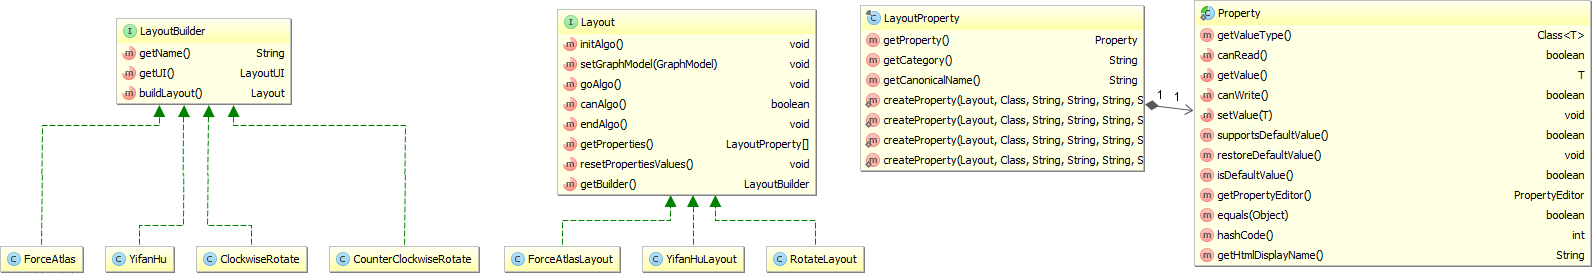
\includegraphics[width=1\textwidth]{images/class-diagram/layout}
 	\caption[Struktura tříd pro výpočet funkcí \uv{Rozložení}]{Struktura tříd pro výpočet funkcí \uv{Rozložení}.}\label{fig:uml-layout}
\end{figure}

\lstinputlisting[caption=Aplikace funkce rozložení \texttt{YifanHu}, firstline=20, lastline=29]{source_code_examples/LayoutExample.java}

\subsubsection{Statistiku a metriky}
Struktura tříd (viz obr. \ref{fig:uml-statistics}) je obdobná jako u \uv{Rozložení}. V tomto případě ale třída \texttt{Statistics} neobsahuje 
žádný seznam možných parametrů. Ty jsou nastavovány přímo z uživatelského rozhraní (implementace rozhraní \texttt{StatisticsUI}) pomocí getterů a settrů.
Seznam parametrů bude tedy nutné získat na základě metod třídy za běhu programu pomocí reflexe.

Výstupem \uv{Statistik} je kromě pozměněného grafu také html zpráva obsahující souhrnné informace o rozložení metrik. Ta je dostupná po
aplikaci metriky pomocí metody \texttt{Statistics::getReport()}.

\begin{figure}\centering
 	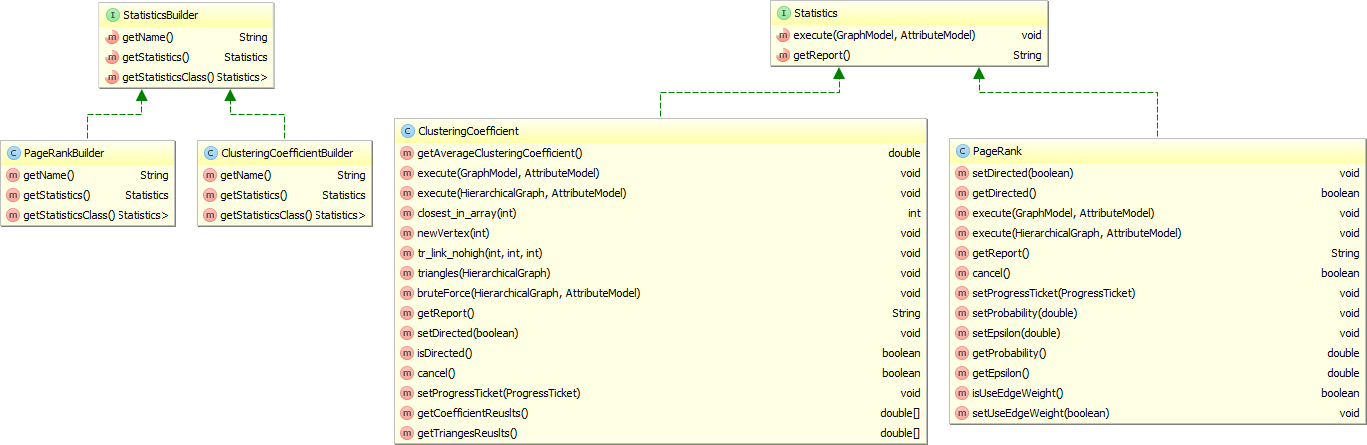
\includegraphics[width=1\textwidth]{images/class-diagram/statistics}
 	\caption[Struktura tříd pro výpočet \uv{Statistik a metrik}]{Struktura tříd pro výpočet \uv{Statistik a metrik}.}\label{fig:uml-statistics}
\end{figure}

\lstinputlisting[caption=Aplikace statistické funkce \texttt{GraphDistance}, firstline=29, lastline=41]{source_code_examples/StatisticsExample.java}

\subsubsection{Filtry}
Základladní třídou pro aplikaci filtrů je třída \texttt{Filter} a k jejímu vytvoření slouží třída \texttt{FilterBuilder} (viz obr. \ref{fig:uml-filter}).
Avšak narozdíl od \uv{Statistik} a \uv{Rozložení}, některé buildery jsou vytvářeny v závislosti na obsahu grafu za pomoci třídy \texttt{CategoryBuilder}.
Například \texttt{AttributeRangeBuilder} (category builder) vytvoří příslušný filter builder pro každý číselný atribut. 

\texttt{Filter} obsahuje seznam parametrů, s jehož pomocí lze jeho konfiguraci snadno vylistovat na nastavit.
Z filtru se následně vytvoří objekt \texttt{Query}, který se aplikuje na graf (viz ukázka kódu \ref{sourcecode:filter}).

\begin{figure}\centering
 	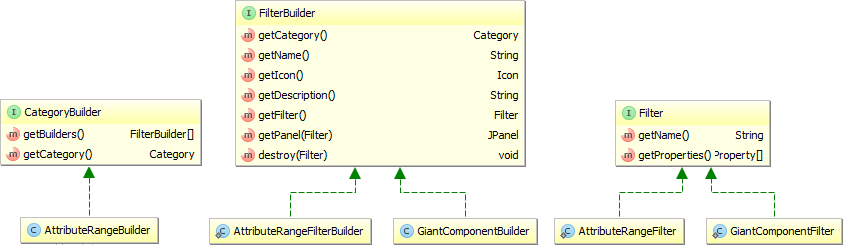
\includegraphics[width=1\textwidth]{images/class-diagram/filter}
 	\caption[Struktura tříd pro výpočet \uv{Statistik a metrik}]{Struktura tříd pro aplikaci \uv{Filtrů}.}\label{fig:uml-filter}
\end{figure}

\lstinputlisting[caption=Aplikace filtru \texttt{GiantComponent}, label=sourcecode:filter, firstline=31, lastline=40]{source_code_examples/FiltersExample.java}

\subsubsection{Hodnocení}
K aplikaci hodnocení slouží třída \texttt{RankingController} a její metoda \texttt{transform\-(Rank\-ing, Trans\-former)}. Stačí jen specifikovat podle čeho hodnotit
a co bude výstupem. K tomu slouží implementace rozhraní \texttt{Ranking} (na základě čeho hodnotit) a \texttt{Transformer}. Jejich implementace můžete vidět na 
obr. \ref{fig:uml-ranking}. Hodnotit lze na základě jakéhokoli atributu uzlu nebo hrany (případně podle stupně uzlu). Výstupem hodnocení může být změna barvy (uzlu, hrany, popisku) 
nebo velikosti (uzlu, hrany).

\begin{figure}\centering
 	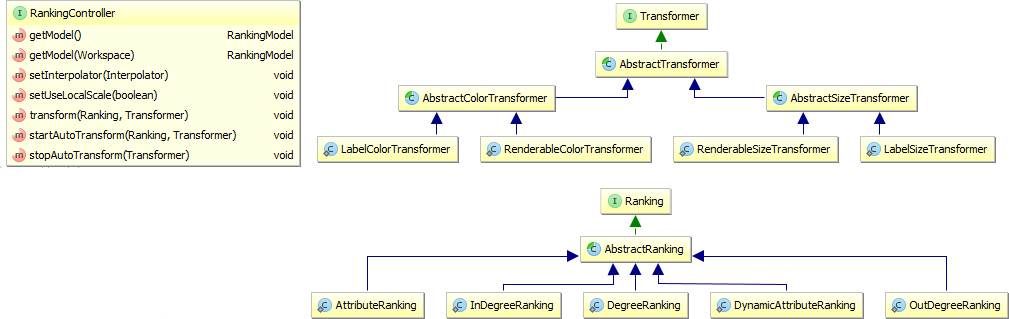
\includegraphics[width=1\textwidth]{images/class-diagram/ranking}
 	\caption[Struktura tříd pro výpočet \uv{Hodnocení}]{Struktura tříd pro výpočet \uv{Hodnocení}.}\label{fig:uml-ranking}
\end{figure}

\lstinputlisting[caption=Změna velikosti uzlu podle hodnoty atributu \uv{betweenesscentrality}, firstline=31, lastline=41]{source_code_examples/RankingExample.java}

\subsection{Seznam dostupných funkcí}
Jak už jsme zmínili, klíčovým požadavkem pro \textit{WebGephi} je schopnost najít všechny dostupné grafové funkce, tzn. všechny implementace
rozhraní \texttt{Layout\-Builder} a \texttt{Statistics\-Builder}. Tento list nemůže být statický. Musíme totiž zároveň zachovat rozšiřitelnost, 
pokud k aplikaci přidáme plugin obsahující např. funkci pro výpočet \uv{Rozložení}, aplikace ho musí sama přidat do svého (REST) rozhraní.

Jelikož nemůžeme využít možností \textit{NetBeans} platformy, musíme využít možností samotného jazyku Java. Pomocí reflexe nalezneme všechny
implementace daných rozhraní (\texttt{LayoutBuilder} a \texttt{StatisticsBuilder}) a s jejich pomocí už máme dostupnou potřebnou funkcionalitu.
Takto nalezneme všechny implementace dostupné na classpath aplikace, je tím tedy zajištěna požadovaná rozšiřitelnost. Z bezpečnostních důvodů
nebude možné přidávat pluginy za běhu aplikace, proces nalezení všech dostupných funkcí tedy bude stačit provést pouze jednou po startu aplikace.

V případě \uv{Hodnocení} se nepočítá s dalším rozšiřováním, tudíž není třeba zjišťovat dostupné možnosti dynamicky. Bude stačit implementovat několik základních možností.
 
\subsection{Víceuživatelský přístup}
Architektura \textit{Gephi} je od počátku navrhována pro potřeby desktopové aplikace. Je z velké části založena na návrhovém vzoru Singleton\footnote{\textit{\uv{Singleton 
(česky jedináček nebo také unikát) je název pro návrhový vzor, používaný při programování. Využijeme ho při řešení problému, kdy je potřeba, aby v celém programu
 běžela pouze jedna instance třídy. Tento návrhový vzor zabezpečí, že třída bude mít jedinou instanci a poskytne k ní globální přístupový bod.}}\cite{wiki:singleton}}. 
 Např. všechny kontrolery jsou singletony. To není v zásadě problém, protože kontrolery nejsou stavové. Problémy nastávají v momentě, kdy chceme pracovat s více Workspace 
 najednou (ve vícevláknovém prostředí). Tento problém je ostatně zmíněn (ne příliš výrazně) i na stránkách s příklady použití \textit{Gephi Toolkit}.
 
 \textit{\uv{(\ldots) many modules just do their job on this current workspace and doesn't allow to specify which workspace to work on from the API. 
 Therefore it is often required to set current workspace, as showed in export here.}\cite{gephi:toolkit}}
 
 Architektura \textit{Gephi} je totiž navržena tak, že vždy právě jeden Projekt a Workspace je aktivní. A přestože některé moduly (třídy, metody) se tváří tak,
 že umí pracovat s Workspace předaným v parametru, v těle metody se používá \uv{current Workspace}. Tento problém ilustruji na příkladu \ref{sourcecode:bug1} třídy \texttt{DefaultProcessor}, která se
 využívá při importu grafu.
 
\lstinputlisting[caption=Import grafu do Workspace\, který není nastavený jako \uv{currentWorkspace}, firstline=31, lastline=37, label=sourcecode:bug1]{source_code_examples/ConcurrencyBugExample.java}
 
 Vše vypadá na první pohled v pořádku, graf se zdánlivě načte do Workspace \texttt{notCurrentWorkspace}. Pokud se však podíváme do implementace třídy \texttt{Default\-Processor} (viz ukázka kódu \ref{sourcecode:bug2}) zjistíme, že 
 se ze skutečnosti používá Workspace nastavený v Singletonu \texttt{ProjectController} jako \uv{currentWorkspace}.

\lstinputlisting[caption=Výřez z implementace třídy \texttt{DefaultProcessor} , firstline=39, lastline=52, label=sourcecode:bug2]{source_code_examples/ConcurrencyBugExample.java}
  
 Tento problém lze vyřešit (jak ostatně zní doporučení v dokumentaci \textit{Gephi Toolkit}) tím, že vždy nastavíme jeden workspace jako \uv{current} a pracujeme pouze s ním.
 To může fungovat u desktopové aplikace, v serverovém prostředí se však pohybujeme ve vícevláknovém prostředí. Museli bychom prakticky veškerou práci s \textit{Gephi Toolkit}
 provádět serializovaně, (v \texttt{synchronized} bloku nebo nějakou pokročilejší technikou zajišťující, že k danému úseku kódu přistupuje vždy jen jedno vlákno). To
 by samozřejmě způsobovalo úzké hrdlo aplikace a výrazně degradovalo výkon. Prakticky by mohl být v jednu chvíli zpracováván vždy jen jeden požadavek.
 V kombinaci s tím, že operace nad grafy mohou trvat relativně dlouho, by se aplikace stala naprosto nepoužitelnou už pro relativně malý počet uživatelů.
 
 Druhé možné řešení je odstranění těchto chyb tím, že upravíme původní třídy tak, abychom místo s \uv{currentWorkspace} pracovali s konkrétním Work\-space předaným komponentě.
 Jedná se o relativně malé množství komponent, tudíž bude toto řešení vhodnější. Tyto třídy budou součástí \textit{WebGephi}, nebude se jednat o úpravy samotné knihovny.
 
\section{Možnosti autentizace a autorizace}
\textit{WebGephi} bude multiuživatelská aplikace. Kdokoli se bude moci založit svůj účet, nahrávat a upravovat své grafy.
Z toho přirozeně plyne nutnost autentizace (ověření identity uživatele) a autorizace (určení, zda má uživatel práva pro danou operaci).

\textit{WebGephi} však bude poskytovat pouze REST rozhraní, které málokdo bude využívat přímo. Místo toho autorizuje nějakou klientskou aplikaci, aby
mohla přistupovat k jeho účtu. Tato aplikace pak skrze vhodné grafické rozhraní umožní uživateli pracovat s jeho grafy.

Zde si představíme standardizovaná řešení této problematiky.

\subsection{Basic autentizace\cite{wiki:basic}}
Basic autentizace je jednou z nejstarších metod autentizace. Princip, jak už název napovídá, je velmi jednoduchý. Klient (většinou webový prohlížeč) zašle
v hlavičce HTTP požadavku své jméno a heslo\footnote{ve formě \texttt{uživatelskéJméno:heslo}, zakódováno pomocí base64}. Server ověří správnost údajů a na jejich základě poskytne nebo
odmítne poskytnout požadovaný obsah.

Pokud požadované přihlašovací údaje chybí, vrátí server odpověď s požadavkem na Basic autentizaci.

\begin{figure}\centering
 	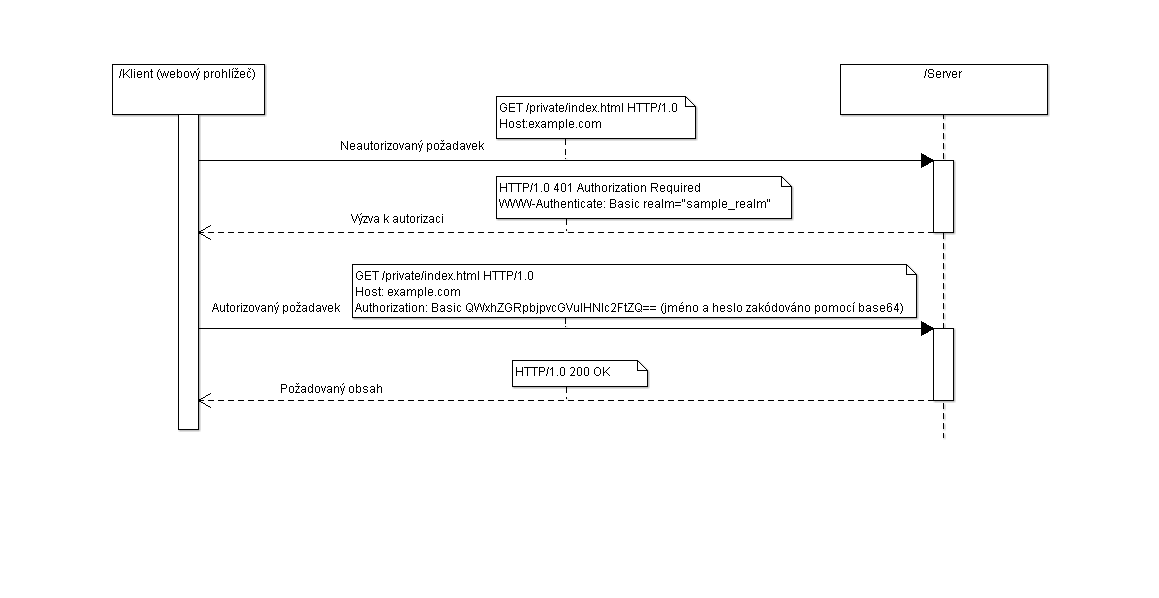
\includegraphics[width=1\textwidth]{images/diagram/auth_basic}
 	\caption[Průběh Basic autorizace]{Průběh Basic autorizace.}\label{fig:auth-basic}
\end{figure}

Výhodou této metody je její jednoduchost. Snad každý HTTP klient obsahuje podporu pro Basic autentizaci. Všechny rozšířené webové prohlížeče si navíc pamatují 
zadané přihlašovací údaje a není tedy nutné je zadávat vždy znovu.

Nevýhodou je, že je nutné zasílat přímo přihlašovací údaje, navíc v nezašifrované podobě a tudíž kdokoli může údaje po cestě odposlechnout. Při použití HTTPS protokolu se však
jedná o bezpečnou metodu autentizace.

\subsubsection{Použití pro WebGephi}
Jedná se o vhodnou metodu pro přímé procházení a prozkoumávání REST rozhraní. Není však vhodné pro poskytování přístupu aplikacím třetích stran (klientské aplikace).
V tomto případě by bylo nutné předat klientské aplikaci přímo své uživatelské jméno a heslo. Tím by uživatel poskytl plný přístup ke svému účtu a nevěrohodná klientská
aplikace by toho mohla zneužít (v krajním případě změnit heslo a tím \uv{ukrást} uživatelův účet). Uživatel by navíc nemohl odebrat aplikaci již jednou udělené oprávnění. 
Pro tento účel by jedině musel změnit své heslo.

Tento způsob autentizace je tedy vhodný jedině pro přímé prozkoumávání REST rozhraní aplikace. Mohl by být použit také v případě,
kdy klientská aplikace využívá jen svůj vlastní účet (může případně řešit správu uživatelů na své straně). 

\subsection{Digest autentizace\cite{wiki:digest}}
Jedná se o mírnou evoluci Basic autentizace. Princip je úplně stejný, v tomto případě se však neposílá heslo přímo, ale jeho hash\footnote{Používá se \texttt{MD5} hash kombinace hesla, cílové uri, metody (GET, POST, \ldots), nonce (serverem 
poskytnutý náhodný řetězec, cnonce (klientův náhodný řetězec) a pořadí požadavku. Více viz \cite{wiki:digest})}.
Z hlediska bezpečnosti se jedná o mírné zlepšení. Při odposlechnutí požadavku nelze (pokud je autentizace správně implementována) požadavek zopakovat.
Nevýhodou je složitější implementace jak na straně serveru, tak na straně klienta.

\subsubsection{Použití pro WebGephi}
Tato metoda, za předpokladu že použijeme HTTPS, nepřináší prakticky žádné výhody oproti Basic autorizaci. Naopak je složitější na implementaci.

\subsection{OAuth v1.0a}
\textit{\uv{Protokol OAuth umožňuje webovým stránkám nebo aplikacím (\textit{Konzumentům}) přistupovat k chráněným zdrojům webových služeb (\textit{Poskytovatele služeb}) skrz API bez nutnosti, aby uživatel
prozradil své přihlašovací údaje k \textit{Poskytovateli služeb} \textit{Konzumentům}. Obecněji, OAuth vytváří volně implementovatelnou a obecnou metodiku pro autentizaci k API}}
\footnote{Volný překlad. Orig.: \textit{\uv{The OAuth protocol enables websites or applications (Consumers) to access Protected Resources from a web service (Service Provider) via an API,
 without requiring Users to disclose their Service Provider credentials to the Consumers. More generally, 
 OAuth creates a freely-implementable and generic methodology for API authentication.}}\cite{oauth:v1}}
 
 OAuth je standardizovaný způsob, jak uživatel může poskytnout přístup ke svému účtu (chráněným zdrojům) u nějaké aplikace (\textit{Poskytovatel služeb}) jiné aplikaci (\textit{Konzument}). A
 to bez toho, aby této aplikaci (\textit{Konzumentovi}) musel prozradit své přihlašovací údaje. Ukázkový příklad pro využití OAuth protokolu je znázorněn na obr. \ref{fig:auth_oauth_example}.

\begin{figure}\centering
 	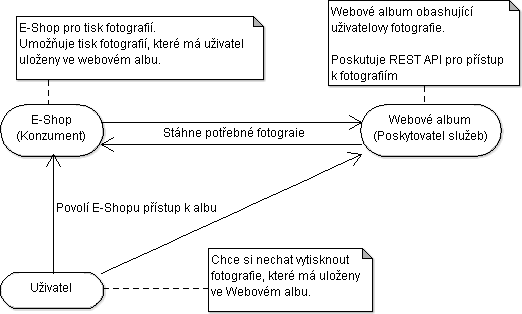
\includegraphics[width=1\textwidth]{images/diagram/auth_oauth_example}
 	\caption[Ukázkový příklad využití OAuth protokolu]{Ukázkový příklad využití OAuth protokolu.}\label{fig:auth_oauth_example}
\end{figure}

\textit{Konzument} musí být zaregistrován u \textit{Poskytovatele služeb} a má svůj jednoznačný identifikátor (\texttt{consumer key}) a heslo (\texttt{consumer secret}).
Pokud požaduje přístup k uživatelovým datům u \textit{Poskytovatele služeb}, zažádá nejdříve o \texttt{Request token}. Ten specifikuje, k jakým zdrojům požaduje aplikace
přístup. Poté přesměruje uživatele na stránky \textit{Poskytovatele služeb}. Uživatel se zde přihlásí a autorizuje požadavek \textit{Konzumenta}, následně je přesměrován 
zpět na stránky \textit{Konzumenta}. Odpověď obsahuje \texttt{verifier}, který \textit{Konzument} použije k výměně \texttt{Request tokenu} za \texttt{Access token}. \texttt{Access token}
už může být použit přímo k přístupu k požadovaným zdrojům. Podrobný popis průběhu OAuth autorizace je znázorněn na obr. \ref{fig:auth-oauth1}.

\begin{figure}\centering
 	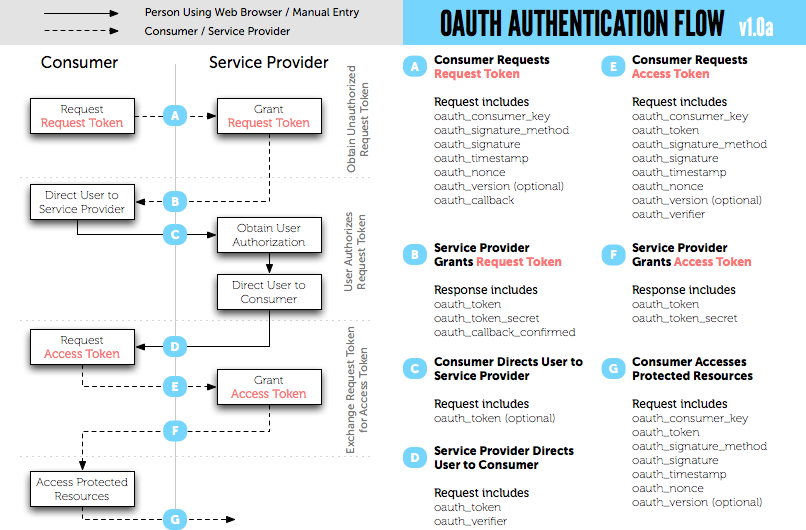
\includegraphics[width=1\textwidth]{images/diagram/auth_oauth1}
 	\caption[Průběh OAuth autorizace]{Průběh OAuth autorizace. Převzato z \cite{oauth:v1}}\label{fig:auth-oauth1}
\end{figure}

Autentizace a autorizace pomocí OAuth v1.0a protokolu je velmi bezpečná. Veškerá komunikace s API \textit{Poskytovatele služeb} je podepisována pomocí informací z 
\texttt{Access tokenu}. Navíc všechny citlivé informace jsou při přenosu šifrovány. To umožňuje jeho bezpečné použití i bez použití SSL. Na druhou stranu je kvůli tomu OAuth náročný na implementaci 
jak na straně serveru, tak na straně klienta. Při použití HTTPS je navíc šifrování v podstatě duplikátní. Na druhou stranu díky přesné specifikaci existují hotové knihovny pro jeho použití.

Hlavní výhodou OAuth protokolu je, že nemusíme aplikacím třetích stran vyzradit své přihlašovací údaje jen kvůli tomu, abychom jim poskytli přístup k části svých chráněných zdrojů. Toto povolení můžeme navíc
kdykoliv odebrat. Protokol také umožňuje poskytnout přístup pouze k části zdrojů (tzv. \texttt{scopes}).

\subsubsection{Použití pro WebGephi}
OAuth je ideální protokol pro \textit{WebGephi}. Jeho součástí je částečně i způsob registrace klientských aplikací. Umožňuje uživatelům udělovat oprávnění klientským aplikacím (\textit{Konzumentům}), aby mohli 
přistupovat k jejich účtům na \textit{WebGephi} (\textit{Poskytovatel služeb}). A to bez toho, aby museli prozradit své přihlašovací údaje. Navíc nemusí udělovat plný přístup
ke svému účtu, některé aplikace mohou např. požadovat pouze práva pro čtení. Typicky žádná aplikace nebude mít práva pro úpravu uživatelova profilu (jména, hesla).

Jedinou nevýhodou je složitější implementace protokolu na straně serveru i klienta.

\subsection{OAuth v2.0\cite{oauth:v2}}
Jedná se o novou verzi, která vyšla v říjnu 2012 (RFC 6749). Již dlouho předtím však byla ve stadiu návrhu. Její cílem bylo zjednodušení protokolu
a větší použitelnost pro jiné než webové aplikace (desktopové, mobilní, \ldots). Hlavní změnou je, že komunikace již není šifrována, plně se spoléhá na SSL šifrování
(nutnost použití společně s HTTPS). Zavádí také více různých způsobů autorizace (kromě klasického \uv{three-legged} OAuth), které jsou vhodné např. pro mobilní aplikace.

Jedná se o volnější specifikaci než je OAuth 1.0a. Jednotlivé implementace se výrazně liší a většinou nejsou spolu kompatibilní.

\subsubsection{Použití pro WebGephi}
OAuth v2.0 nepřináší oproti první verzi z pohledu \textit{WebGephi} žádné výrazné výhody. Volnější specifikace a nekompatibilita jednotlivých implementací ztěžuje 
jeho použití různými \textit{Konzumenty}. Výhodou by byla lepší podpora desktopových a mobilních klientů.

\subsection{Výběr autentizace a autorizace pro WebGephi}
Pro \textit{WebGephi} byla vybrána kombinace Basic autorizace a OAuth v1.0a. Preferována bude OAuth autorizace, která umožňuje bezpečnější a přesnější řízení přístupu.
Basic autorizace se bude používat pouze pro prozkoumávání a vyzkoušení REST rozhraní a v případech, kdy klientská aplikace není (kvůli složitosti) schopná implememtovat OAuth klienta.
To se může stát např. v případě čistě JavaScriptového klienta.

\chapter{Návrh}
V kéto kapitole se zaměříme na návrh struktury aplikace \textit{WebGephi}. Představíme si základní workflow aplikace a její datový model.
Nejdůležitější částí kapitoly bude popis REST API. Protože výsledná aplikace nebude monolitická, popíšeme si zde také význam jednotlivých 
modulů.

\section{Procesní model}

Na diagramu \ref{fig:webgephi-workflow} je znázorněno, jak bude řešeno základní workflow ve \textit{WebGephi}. Základem je úložiště uživatelových 
grafů. Na tyto grafy může klient aplikovat dostupné grafové funkce (\texttt{Layout}, \texttt{Statistics}, \texttt{Ranking}). Po každé aplikaci funkce
se výsledek uloží jako nový graf a uživateli se vrátí odkaz na něj. To mimo jiné umožní zobrazenit historii práce s každým grafem.

Vytvořené grafy nebude možné mazat ani upravovat. To umožní snadnou kešovatelnost úložiště. 

\begin{figure}\centering
 	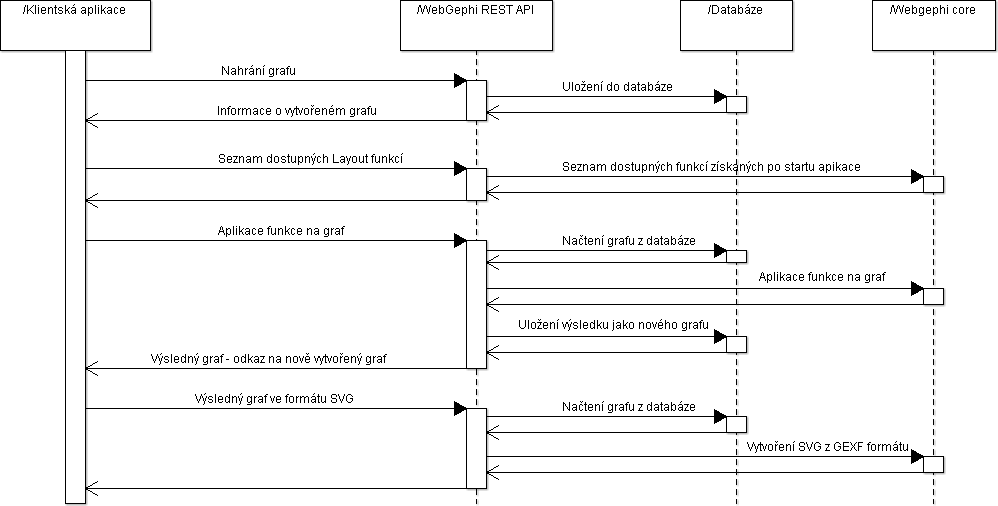
\includegraphics[width=1\textwidth]{images/diagram/webgephi_workflow}
 	\caption[Sekvenční diagram práce s WebGephi]{Sekvenční diagram práce s WebGephi}\label{fig:webgephi-workflow}
\end{figure}

\section{Datový model}
Datový model aplikace bude velmi jednoduchý (viz diagram \ref{fig:webgephi-dbmodel}). Zde si popíšeme jeho jednotlivé prvky.

\begin{figure}\centering
 	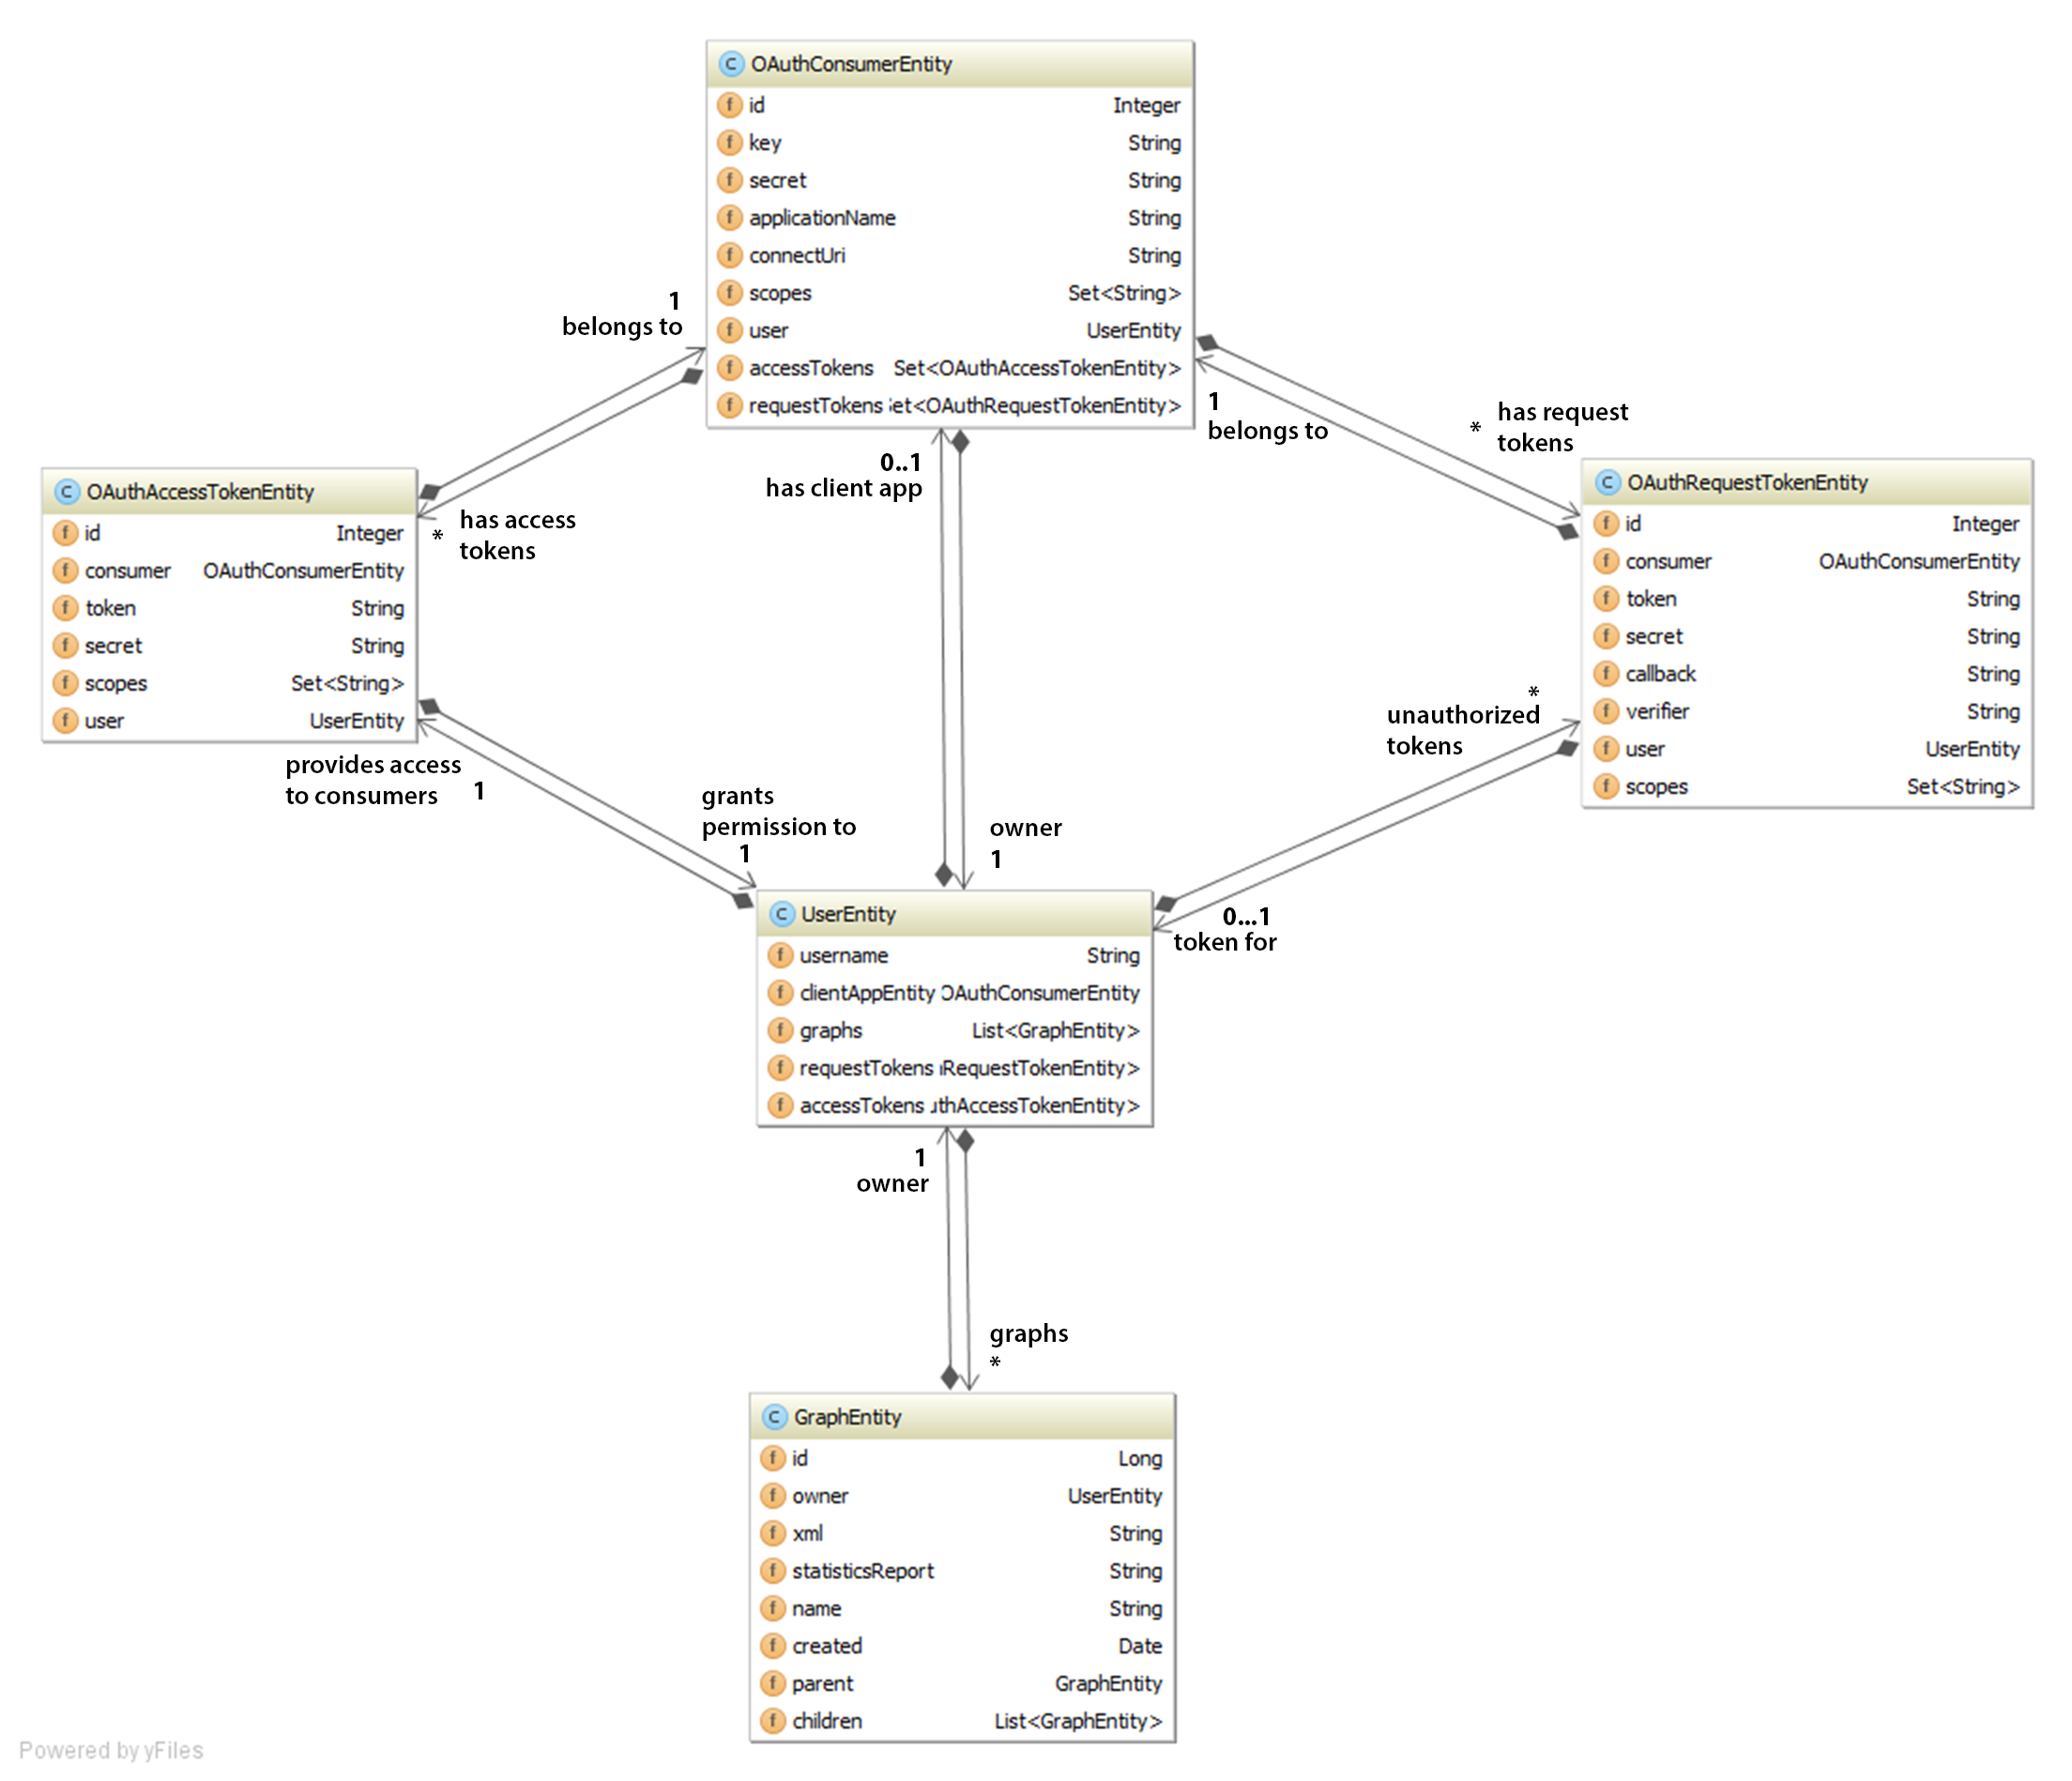
\includegraphics[width=1\textwidth]{images/class-diagram/db_model}
 	\caption[Datový model WebGephi]{Datový model WebGephi}\label{fig:webgephi-dbmodel}
\end{figure}

\subsection{User}
Entita \texttt{User} představuje běžného uživatele aplikace (případně admina, struktura rolí není v modelu znázorněna). Každý
uživatel má přístup ke svým grafům a může spravovat jednu klientskou aplikaci.

\subsection{Graph}
Entita graph představuje jeden graph, jeho struktura je uložena ve formátu \texttt{gexf}. Pokud byla na graf aplikována statistická funkce,
v atributu \texttt{statistics\-Report} je uložena shrnující zpráva (formát \texttt{html}). Kromě toho má každý graf své jméno a informaci 
o datu vytvoření.

\subsection{OAuth}
Pro potřeby OAuth autorizace musí datový model také obsahovat potřebné informace. Jedná se o entity \texttt{OAuth\-Consumer}, \texttt{OAuth\-Access\-Token} a \texttt{OAuth\-Request\-Token}.

\subsubsection{OAuthConsumer}
Tato entita představuje klientskou aplikaci (v OAuth termnologii se jedná o \textit{Konzumenta}). Pro její vytvoření a správu musí být přiřazena k uživateli, který je pak její správce (vlastník).
\textit{Konzument} pak může od uživatelů požadovat přístup k jejich účtu.

\subsubsection{OAuthRequestToken}
Jedná se o dočasnou entitu potřebnou pro zažádání přístupu k cizímu účtu. Po autorizaci tokenu uživatele je \texttt{Request token} smazán a nahrazen \texttt{Access tokenem}.

\subsubsection{OAuthAccessToken}
Představuje udělené oprávnění pro \textit{Konzumenta} přistupovat k účtu jiných uživatelů. Kromě identifikátoru (atribut \texttt{token}) a tajného klíče (atribut \texttt{secret}) obsahuje také seznam
oprávnění, které token poskytuje (atribut \texttt{scopes}).

Uživatel může kdykoli smazat \texttt{Access token} a tím zrušit udělěné oprávnění.

\section{REST rozhraní}
Rozhraní aplikace \textit{WebGephi} bude vytvořeno jako RESTful\footnote{Webová služba splňující principy REST architektury} webová služba. REST architektura je 
založena na \textit{zdrojích (resources)}. Každá URI představuje zdroj a webová služba poskutuje standardní metody pro práci s nimi. V případě použití protokolu HTTP (naprostá většina RESTful služeb) se 
používají přímo metody tohoto protokolu.

\subsection{Metody RESTful webových služeb}
\begin{description}
  \item[GET] Zobrazení konkrétní rerezentace zdroje
  \item[POST] Vytvoření nového objektu - zdroje. Data jsou odesílána v tělě požadavku. 
  \item[PUT] Úprava existujícího zdroje na základě dat v těle požadavku.
  \item[DELETE] Smazání existujícího zdroje.
  \item[HEAD] Popis formátu zdroje.
\end{description}
 

\subsection{Struktura WebGephi REST rozhraní}
Zde podrobně popíšeme struktury RESTful webové služby \textit{WebGephi}. Základní struktura je znázorněna diagramu \ref{fig:webgephi-restful}

\begin{figure}
	\dirtree{%
		.1 \{api\_version\}.
			.2 users:GET\DTcomment{Zobrazení seznamu všech uživatelů}.		  		
				.3 \{username\}\DTcomment{Uživatel \uv{username}}.
					.4 :GET\DTcomment{Zobrazení}.
					.4 :POST\DTcomment{Přidání}.
					.4 :PUT\DTcomment{Editace}.
					.4 graphs:GET\DTcomment{Zobrazení všech grafů uživatele}.			
						.5 \{graph\_id\}\DTcomment{Graf s id \uv{graph\_id} (id, jméno, datum)}.
							.6 :GET\DTcomment{Zobrazení}.
							.6 :POST\DTcomment{Přidání nového grafu}.
							.6 :PUT\DTcomment{Aplikace funkce na graf}.
							.6 gexf:GET\DTcomment{graf ve formátu gexf}.
							.6 svg:GET\DTcomment{graf ve formátu svg}.
							.6 statistics-report:GET\DTcomment{zpráva o výsledku statistické funkce (html)}.
			.2 layouts:GET\DTcomment{Seznam všech dostupných funkcí pro výpočet rozložení}.
				.3 \{layout\_id\}:GET\DTcomment{Detail funkce}.
			.2 statistics:GET\DTcomment{Seznam všech dostupných statistických funkcí}.
				.3 \{statistic\_id\}:GET\DTcomment{Detail funkce}.
			.2 rankings:GET\DTcomment{Seznam všech dostupných funkcí pro hodnocení}.
				.3 \{ranking\_id\}:GET\DTcomment{Detail funkce}.
			.2 filters:GET\DTcomment{Seznam všech dostupných filtrů}.
				.3 \{filter\_id\}:GET\DTcomment{Detail filtru}.
	}
	\caption[Struktura zdrojů RESTful služby \textit{WebGephi}]{}\label{fig:webgephi-restful}
\end{figure}

U každého zdroje je popsán popis možných parametrů a obsah těla požadavku a odpovědi. Pokud během zpracování požadavku
dojede k nějaké nestandardní situaci (data požadavku jsou nevalidní, interní chyba systému, \ldots), místo standarní 
odpovědi s kódem 200 (OK) je vrácena odpověď s příslušným HTTP kódem a popisem problému (viz \ref{rest:error-xml}).

\begin{lstlisting}[caption=XML a HTML chybová odpověď, label=rest:error-xml, language=xml]
<error>
    <code number="409">Conflict</code>
    <message>User is invalid</message>
    <detail>Username test is already taken.</detail>
</error>

<html>
<head>
    <title>Error 404 (Not Found)</title>
</head>
<body>
    <h1>404 (Not Found)</h1>
    <ul>
        <li>Message: This graph has no statistics</li>
        <li>Detail: Statistics are set only if some statistic function was applied previously</li>
    </ul>
</body>
</html>
\end{lstlisting}


\subsubsection{Seznam dostupných funkcí pro výpočet rozložení}
\begin{description}
  \item[URI]\footnote{Všechny URI jsou relativní k \{server\_url\}/rest/v1/} /layouts
  \item[Metoda] GET
  \item[Potřebné oprávnění]\footnote{viz sekce \ref{roles}} Žádné
  \item[Tělo požadku] Prázdné
  \item[Tělo odpovědi] Seznam \uv{Layout} funkcí dostupných v systému (ukázka \ref{rest:resp:layouts}).
\end{description}

\begin{lstlisting}[caption=Tělo odpovědi zdroje /layouts (GET), label=rest:resp:layouts, language=xml]
<layouts>
   <layout id="clockwise-rotate">
      ...
   </layouts>
   ...
</layouts>
\end{lstlisting}  

\subsubsection{Detail funkce pro výpočet rozložení}
\begin{description}
  \item[URI] /layouts/\{layout\_id\}
  \item[Metoda] GET
  \item[Potřebné oprávnění] Žádné
  \item[Tělo požadku] Prázdné
  \item[Tělo odpovědi] Popis konkrétní fukce (jméno, parametry, \ldots) (ukázka \ref{rest:resp:layout}).
\end{description}

\begin{lstlisting}[caption=Tělo odpovědi zdroje /layouts/\{layout\_id\} (GET), label=rest:resp:layout, language=xml]
<layout id="clockwise-rotate">
    <name>Clockwise Rotate</name>
    <properties>
        <property id="clockwise.angle.name">
            <name>Angle</wg:name>
            <description>Clockwise rotation angle in degrees</wg:description>
            <value>
                <double value="90.0"/>
            </value>
        </property>
    </properties>   
</layout>
\end{lstlisting}    

\subsubsection{Seznam dostupných statistických funkcí}
\begin{description}
  \item[URI] /statistics
  \item[Metoda] GET
  \item[Potřebné oprávnění] Žádné
  \item[Tělo požadku] Prázdné
  \item[Tělo odpovědi] Seznam statistických funkcí dostupných v systému (ukázka \ref{rest:resp:statistics}).
\end{description}

\begin{lstlisting}[caption=Tělo odpovědi zdroje /statistics (GET), label=rest:resp:statistics, language=xml]
<statistics>
   <statistic id="clustering-coefficient">
      ...
   </statistic>
   ...
</statistics>
\end{lstlisting}  

\subsubsection{Detail statistické funkce}
\begin{description}
  \item[URI] /statistics/\{statistic\_id\}
  \item[Metoda] GET
  \item[Potřebné oprávnění] Žádné
  \item[Tělo požadku] Prázdné
  \item[Tělo odpovědi] Popis konkrétní fukce (jméno, parametry, \ldots) (ukázka \ref{rest:resp:statistic}).
\end{description}

\begin{lstlisting}[caption=Tělo odpovědi zdroje /statistics/\{statistic\_id\} (GET), label=rest:resp:statistic, language=xml]
<statistic id="clustering-coefficient">
   <name>Clustering Coefficient</name>
   <properties>
      <property id="Directed">
            <name>Directed</wg:name>
            <value>
                <boolean value="false"/>
            </value>
        </property>
   </properties>
</statistic>
\end{lstlisting}  

\subsubsection{Seznam dostupných filtrů}
\begin{description}
  \item[URI] /filters
  \item[Metoda] GET
  \item[Potřebné oprávnění] Žádné
  \item[Tělo požadku] Prázdné
  \item[Tělo odpovědi] Seznam filtrů dostupných v systému (ukázka \ref{rest:resp:filters}).
\end{description}

\begin{lstlisting}[caption=Tělo odpovědi zdroje /filters (GET), label=rest:resp:filters, language=xml]
<filters>
   <filter id="attribute-non-null-filter">
      ...
   </filter>
   ...
</filters>
\end{lstlisting}  

\subsubsection{Detail filtru}
\begin{description}
  \item[URI] /filters/\{filter\_id\}
  \item[Metoda] GET
  \item[Potřebné oprávnění] Žádné
  \item[Tělo požadku] Prázdné
  \item[Tělo odpovědi] Popis konkrétního filtru (jméno, parametry, \ldots) (ukázka \ref{rest:resp:filter}).
\end{description}

\begin{lstlisting}[caption=Tělo odpovědi zdroje /fiters/\{filter\_id\} (GET), label=rest:resp:filter, language=xml]
<filter id="attribute-non-null-filter">
    <description>
        Category: Non-null-Attributes; Keep nodes/edges with non-null values for a particular column
    </description>
    <name>Attribute Non Null Filter</name>
    <properties>
        <property id="attribute">
            <name>Attribute column</name>
            <description>Select attribute to filter</description>
            <value>
                <attribute attributeId="column"/>
            </value>
        </property>
    </properties>    
</filter>
\end{lstlisting}  

\subsubsection{Seznam dostupných funkcí pro hodnocení}
\begin{description}
  \item[URI] /rankings
  \item[Metoda] GET
  \item[Potřebné oprávnění] Žádné
  \item[Tělo požadku] Prázdné
  \item[Tělo odpovědi] Seznam funkcí pro hodnocení (ukázka \ref{rest:resp:rankings}).
\end{description}

\begin{lstlisting}[caption=Tělo odpovědi zdroje /rankings (GET), label=rest:resp:rankings, language=xml]
<rankings>
   <ranking id="color-ranking">
      ...
   </ranking>
   ...
</rankings>
\end{lstlisting}  

\subsubsection{Detail funkce hodnocení}
\begin{description}
  \item[URI] /rankings/\{ranking\_id\}
  \item[Metoda] GET
  \item[Potřebné oprávnění] Žádné
  \item[Tělo požadku] Prázdné
  \item[Tělo odpovědi] Popis konkrétní fukce (jméno, parametry, \ldots) (ukázka \ref{rest:resp:ranking}).
\end{description}

\begin{lstlisting}[caption=Tělo odpovědi zdroje /rankings/\{ranking\_id\} (GET), label=rest:resp:ranking, language=xml]
<ranking id="edgeColor">
    <description>
        Ranking according to edge attribute, changes edge color.
    </description>
    <name>Edge color ranking</name>
    <properties>
        <property id="edgeAttribute">
            <name>Edge attribute</name>
            <description>
                Id of attribute which will be used for ranking. It has to be one of already calculated edge attributes (see GEXF format)
            </description>
            <value>
                <edgeAttribute attributeId="id-of-attribute-column"/>
            </value>
        </property>
        <property id="startColor">
            <name>Start color</name>
            <description>
                Color of node with lowest value. In hexadecimal format: RRGGBB, e.g. FEF0D9
            </description>
            <value>
                <color>FEF0D9</color>
            </value>
        </property>
        <property id="endColor">
            <name>End color</name>
            <description>
                Color of node with highest value. In hexadecimal format: RRGGBB, e.g. B30000
            </description>
            <value>
                <color>B30000</color>
            </value>
        </property>
    </properties>
</ranking>
\end{lstlisting}  

\subsubsection{Seznam uživatelů}
Zobrazí seznam všech uživatelů. Tento resource je dostupný pouze pro správce.
\begin{description}
  \item[URI] /users
  \item[Metoda] GET
  \item[Potřebné oprávnění] ADMIN
  \item[Tělo požadku] Prázdné
  \item[Tělo odpovědi] Seznam všech uživatelů v systému (ukázka \ref{rest:resp:users-get}).
\end{description}

\begin{lstlisting}[caption=Tělo odpovědi zdroje /users (GET), label=rest:resp:users-get, language=xml]
<users>
   <user username="admin">
      ...
   </user>
   ...
</users>
\end{lstlisting}  

\subsubsection{Přidání uživatele do systému}
Přidá nového uživatele do aplikace. Vytvořený uživatel bude mít roli USER (bežný uživatel)
\begin{description}
  \item[URI] /users
  \item[Metoda] POST
  \item[Potřebné oprávnění] Žádné
  \item[Tělo požadku] Údaje o uživateli (ukázka \ref{rest:req:users-post})
  \item[Tělo odpovědi] Nově vytvořený uživatel (ukázka \ref{rest:resp:users-post}).
\end{description}

\begin{lstlisting}[caption=Tělo požadavku zdroje /users (POST), label=rest:req:users-post, language=xml]
<user username="test">
    <email>test@test.cz</email>
    <firstName>John</firstName>
    <lastName>Doe</lastName>
    <password>password</password>
</user>
\end{lstlisting}  

\begin{lstlisting}[caption=Tělo odpovědi zdroje /users (POST), label=rest:resp:users-post, language=xml]
<user username="test">
    <email>test@test.cz</email>
    <firstName>John</firstName>
    <lastName>Doe</lastName>
</user>
\end{lstlisting}

\subsubsection{Detail uživatele}
Zobrazí profil uživatele. Heslo se nikdy nezobrazuje.
\begin{description}
  \item[URI] /users/\{username\}
  \item[Metoda] GET
  \item[Potřebné oprávnění] PROFILE\_READ
  \item[Tělo požadku] Prázdné
  \item[Tělo odpovědi] Profil uživatele \texttt{username} (ukázka \ref{rest:resp:user-get}).
\end{description}

\begin{lstlisting}[caption=Tělo odpovědi zdroje /users/\{username\} (GET), label=rest:resp:user-get, language=xml]
<user username="test">
    <email>test@test.cz</email>
    <firstName>John</firstName>
    <lastName>Doe</lastName>
</user>
\end{lstlisting}  

\subsubsection{Přihlášený uživatel}
Zobrazí profil právě přihlášeného uživatele. Slouží klientským aplikacím, aby mohli zjistit, s jakým účtem právě pracují.
\begin{description}
  \item[URI] /users/logged
  \item[Metoda] GET
  \item[Potřebné oprávnění] PROFILE\_READ
  \item[Tělo požadku] Prázdné
  \item[Tělo odpovědi] Profil právě přihlášeného uživatele.
\end{description}

\subsubsection{Editace uživatele}
Upraví profil uživatele podle zadaných informací.
\begin{description}
  \item[URI] /users/\{username\}
  \item[Metoda] PUT
  \item[Potřebné oprávnění] PROFILE\_WRITE
  \item[Tělo požadku] Údaje ke změně \ref{rest:req:user-put})
  \item[Tělo odpovědi] Uživatel po editaci (ukázka \ref{rest:resp:user-put}).
\end{description}

\begin{lstlisting}[caption=Tělo požadavku zdroje /users/\{username\} (PUT), label=rest:req:user-put, language=xml]
<user username="test">
    <email>changed@changed.cz</email>
    <firstName>CHANGED John</firstName>
    <lastName>CHANGED Doe</lastName>
    <password>password2</password>
</user>
\end{lstlisting}  

\begin{lstlisting}[caption=Tělo odpovědi zdroje /users/\{username\} (PUT), label=rest:resp:user-put, language=xml]
<user username="test">   
    <email>changed@changed.cz</email>
    <firstName>CHANGED John</firstName>
    <lastName>CHANGED Doe</lastName>
</user>
\end{lstlisting}

\subsubsection{Seznam grafů uživatele}
Zobrazí seznam všech grafů daného uživatele. Seznam je stránkovaný, stránkování lze řídit pomocí parametrů.
\begin{description}
  \item[URI] /users/\{username\}/graphs?[page=X]\&[pageSize=Y]\&[desc=B]
  \begin{description}
     \item[page] číslo stránky. Výchozí hodnota je 1.
     \item[pageSize] velikost jedné stránky. Výchozí hodnota je 50. 1 <= Y <= 50.
     \item[page] řazení seznamu. Výchozí je false (vzestupně, nejstarší první).
  \end{description}	
  \item[Metoda] GET
  \item[Potřebné oprávnění] GRAPHS\_READ
  \item[Tělo požadku] Prázdné
  \item[Tělo odpovědi] Seznam grafů uživatele (ukázka \ref{rest:resp:graphs-get}).
\end{description}

\begin{lstlisting}[caption=Tělo odpovědi zdroje /users/\{username\}/graphs (GET), label=rest:resp:graphs-get, language=xml]
<graphs>
   <graph id="69">
      ...
   </graph>
   ...
</graphs>
\end{lstlisting}  

\subsubsection{Detail grafu}
Zobrazí detail grafu s daným id. Graf může obsahovat odkaz na rodičovský graf, ze kterého vynikl. To umožňuje zobrazení historii editace grafu.
\begin{description}
  \item[URI] /users/\{username\}/graphs/\{graph\_id\}
  \item[Metoda] GET
  \item[Potřebné oprávnění] GRAPHS\_READ
  \item[Tělo požadku] Prázdné
  \item[Tělo odpovědi] Detail grafu (ukázka \ref{rest:resp:graph-get}).
\end{description}

\begin{lstlisting}[caption=Tělo odpovědi zdroje /users/\{username\}/graphs/\{graph\_id\} (GET), label=rest:resp:graph-get, language=xml]
<graph>
   <created>2014-04-19T19:09:20+02:00</created>
   <name>
      Missereables_clockwise-rotate_force-atlas_force-atlas_page-rank
   </name>
   <parent id="59">
      <created>2014-04-19T19:09:05+02:00</created>
      <name>
         Missereables_clockwise-rotate_force-atlas_force-atlas
      </name>
   </parent>
</graph>
\end{lstlisting}  

\subsubsection{Vytvoření nového grafu}
Přidá nový graf do úložiště. Parametr name určuje jméno vytvořeného grafu.
\begin{description}
  \item[URI] /users/\{username\}/graphs[?name=\{graph\_name\}]
  \item[Metoda] POST
  \item[Potřebné oprávnění] GRAPHS\_WRITE
  \item[Tělo požadku] Graf ve formátu \texttt{gexf} (ukázka \ref{rest:req:graph-post}).
  \item[Tělo odpovědi] Detail vytvořeného grafu.
\end{description}

\begin{lstlisting}[caption=Tělo požadavku zdroje /users/\{username\}/graphs (POST), label=rest:req:graph-post, language=xml]
<gexf version="1.2" xmlns="http://www.gexf.net/1.2draft" ...>
   ...
</gexf>
\end{lstlisting} 

\subsubsection{Graf ve formátu \texttt{gexf}}
Zobrazí graf v datovém formátu \texttt{gexf}.
\begin{description}
  \item[URI] /users/\{username\}/graphs/\{graph\_id\}/gexf
  \item[Metoda] GET
  \item[Potřebné oprávnění] GRAPHS\_READ
  \item[Tělo požadku] Prázdné
  \item[Tělo odpovědi] Reprezentace grafu ve formátu texttt{gexf}.
\end{description}

\subsubsection{Graf ve formátu \texttt{svg}}
Zobrazí graf v grafickém formátu \texttt{svg}.
\begin{description}
  \item[URI] /users/\{username\}/graphs/\{graph\_id\}/svg
  \item[Metoda] GET
  \item[Potřebné oprávnění] GRAPHS\_READ
  \item[Tělo požadku] Prázdné
  \item[Tělo odpovědi] Reprezentace grafu ve formátu texttt{svg} (ukázka \ref{rest:resp:graph-svg}). 
\end{description}

\begin{lstlisting}[caption=Tělo odpovědi zdroje /users/\{username\}/graphs/\{graph\_id\}/svg (GET), label=rest:resp:graph-svg, language=xml]
<svg contentScriptType="text/ecmascript" width="1026px"
     xmlns:xlink="http://www.w3.org/1999/xlink" zoomAndPan="magnify"
     contentStyleType="text/css" viewBox="-537 -514 1269 1040" height="841px"
     preserveAspectRatio="xMidYMid meet" xmlns="http://www.w3.org/2000/svg"
     version="1.1">
     ...
</svg>
\end{lstlisting}  

\subsubsection{Zpráva z výsledků statistické funkce}
Zobrazí HTML zprávu, která je výsledkem aplikace statistické funkce. Dostupné pouze pokud poslední aplikovanou funkcí byla statistická funkce.
\begin{description}
  \item[URI] /users/\{username\}/graphs/\{graph\_id\}/statistics-report
  \item[Metoda] GET
  \item[Potřebné oprávnění] GRAPHS\_READ
  \item[Tělo požadku] Prázdné
  \item[Tělo odpovědi] HTML obsahující zprávu, většinou ve formě grafu rozložení hodnot. 
\end{description}


\subsubsection{Aplikace funkce na graf \texttt{svg}}
Aplikuje funkci na graf (\texttt{Layout}, \texttt{Statistics} nebo \texttt{Ranking}). Výsledek je uložen jako nový graf a vrácen uživateli. 
\begin{description}
  \item[URI] /users/\{username\}/graphs/\{graph\_id\}
  \item[Metoda] PUT
  \item[Potřebné oprávnění] GRAPHS\_WRITE
  \item[Tělo požadku] Definice funkce (ukázka \ref{rest:req:graph-apply-func}).
  \item[Tělo odpovědi] Detail nově vytvořeného grafu. 
\end{description}


\begin{lstlisting}[caption=Tělo požadavku zdroje /users/\{username\}/graphs/\{graph\_id\} (PUT), label=rest:req:graph-apply-func, language=xml]
<function xmlns="" xmlns:xs="http://www.w3.org/2001/XMLSchema" xmlns:xsi="http://www.w3.org/2001/XMLSchema-instance">
    <statistic id="clustering-coefficient">
        <name>Clustering Coefficient</name>
		<properties>
			<property id="Directed">
				<name>Directed</name>
				<value>
					<boolean value="false"/>
				</value>
			</property>
		</properties>
    </statistic>
</function>
\end{lstlisting}  

\section{Autentizace a autorizace}\label{roles}
\textit{WebGephi} bude poskytovat dvě různá rozhraní pro interakci s uživateli:
grafické rozhraní pro správu uživatelů a klientských aplikací a REST webové služby pro práci s grafy (viz diagram. \ref{fig:server-auth}).
K oběma rozhraním bude řízen přístup na základě uživatelských oprávnění a rolí. Autentizace bude v případě REST rozhraní umožněna metodou Basic a OAuth protokolu.
Přihlašování ke grafické části aplikace bude realizováno klasicky pomocí jména a hesla (tzv. Form autentizace).

\begin{figure}\centering
 	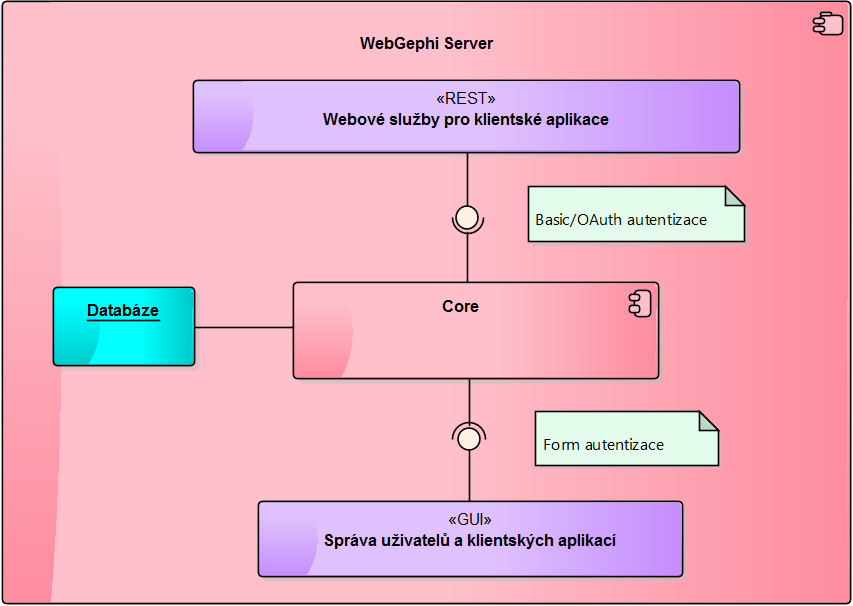
\includegraphics[width=1\textwidth]{images/diagram/server-auth}
 	\caption[Struktura WebGephi]{Struktura WebGephi}\label{fig:server-auth}
\end{figure}

\subsection{Uživatelská oprávnění a role}
Přístup k jednotlivým zdrojům aplikace bude řízen pomocí uživatelských oprávnění. Pokud přihlášený uživatel nebude mít potřebná práva,
bude mu přístup ke zdroji zamezen. Skupiny oprávnění budou sdruženy do rolí, které představují kategorii uživatelů.

\subsubsection{Oprávnění}
Každé oprávnění umožňuje přístup k jednomu typu operace (zdroje).
\begin{description}
  \item[PROFILE\_READ] Čtení profilu přihlášeného uživatele
  \item[PROFILE\_WRITE] Editace profilu přihlášeného uživatele
  \item[GRAPHS\_READ] Zobrazení všech grafů aktuálně přihlášeného uživatele
  \item[GRAPHS\_WRITE] Přidání nového grafu a editace grafů (aplikace funkcí) přihlášeného uživatele 
  \item[ALL\_PROFILES\_READ] Zobrazení všech uživatelů v aplikaci 
  \item[ALL\_PROFILES\_WRITE] Editace jakéhokoliv uživatele v aplikaci 
\end{description}

\subsubsection{Role}
Role představuje skupinu oprávnění. Role uživatele bude určena při přihlášení na základě typu účtu a způsobu přihlášení.
\begin{description}
  \item[ADMIN] Správce stránek. Platná pouze pro Basic a Form autentizaci. Obsahuje všechna dostupná oprávnění: \texttt{PROFILE\_READ}, \texttt{PROFILE\_WRITE}, 
  \newline \texttt{GRAPHS\_READ}, \texttt{GRAPHS\_WRITE}, \texttt{ALL\_PROFILES\_READ}, \texttt{ALL\_PROFILES\_WRITE}.
  \item[USER] Běžný uživatel aplikace, pokud je přihlášen pomocí jména a hesla (Form nebo Basic metodou). Má oprávnění editovat své vlastní zdroje (\texttt{PROFILE\_READ}, \texttt{PROFILE\_WRITE}, \texttt{GRAPHS\_READ}, \texttt{GRAPHS\_WRITE}).
  \item[CLIENT\_APP] Role pro klientské aplikace, tzn. pro uživatele přihlášeného z jiné aplikace přes protokol OAuth. Klientská aplikace může požadovat oprávnění \texttt{PROFILE\_READ}, \texttt{GRAPHS\_READ} a \texttt{GRAPHS\_WRITE} (tzv. \uv{scopes} v OAuth terminologii). Požadovaná oprávnění se uživateli zobrazí při zobrazení žádosti o udělení přístupu (potvrzení \texttt{Request tokenu}). Některé klientské aplikace mohou např. požadovat pouze práva ke čtení grafů, jiné i k editaci grafu a zobrazení informací o uživateli. Uživatel vždy uvidí jaká práva aplikace požaduje a na základě toho se rozhodne, zda jí přístup udělí.
\end{description}

\section{Správa uživatelů a klientských aplikací}
Správa uživatelů a klientských aplikací bude realizována pomocí grafického rozhraní. Základní správa uživatelských účtů bude navíc umožněna pomocí REST webových služeb.
Předpokládáme dva základní případy užití\footnote{Use-case} (viz obr. \ref{fig:sprava_uzivatelu-use_cases}).

\begin{figure}\centering
 	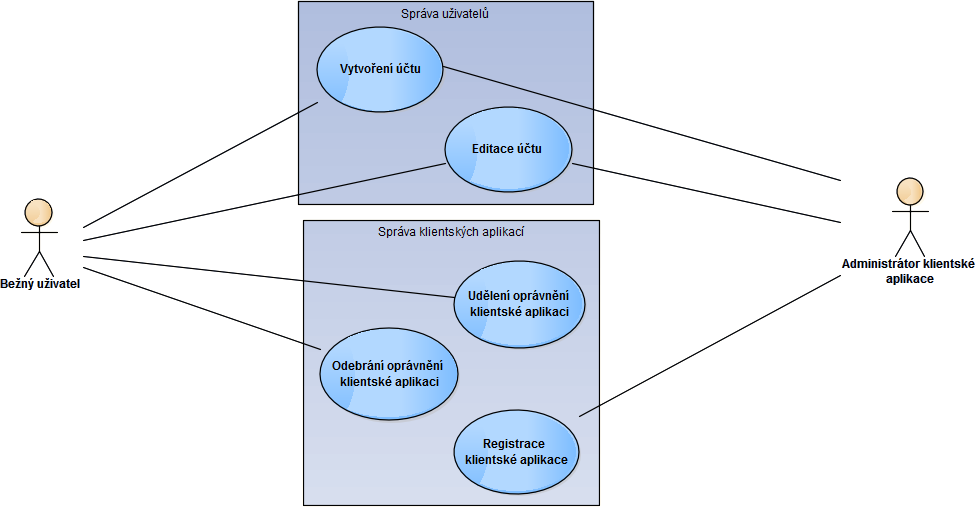
\includegraphics[width=1\textwidth]{images/diagram/sprava_uzivatelu-use_cases}
 	\caption[Případy užití uživatelského účtu]{Případy užití uživatelského účtu}\label{fig:sprava_uzivatelu-use_cases}
\end{figure}

\subsection{Běžný uživatel}
Běžný uživatel je na WebGephi přesměrován z klientské aplikace. Založí si zde uživatelský účet, čímž získá možnost vytvářet a editovat vlastní grafy. To však nedělá přímo,
místo toho udělí právo  přístupu klietské aplikaci (pomocí OAuth protokolu). Tato oprávnění může kdykoli odebrat.

\subsection{Administrátor klientské aplikace}
Jedná se o správce, případně vývojáře nějaké aplikace, která chce využívat možností WebGephi. Nejdříve si musí založit běžný účet. V rámci svého
uživatelského účtu si zaregistruje svou klientskou aplikaci, čímž získá potřebné informace pro přihlášování pomocí OAuth protokolu (\texttt{consumer\_key} a \texttt{consumer\_secret}).
Následně může ze své aplikace od uživatelů požadovat přístup k jejich účtu na WebGephi.

\section{Struktura aplikace}
Cílem této práce je kromě vytvoření serverové aplikace také vytvoření ukázkové klientské aplikace. V této kapitole si popíšeme strukturu a
závislosti těchto aplikací a jejich modulů. Základní struktura je znázorněma na obr. \ref{fig:modules}.

\begin{figure}\centering
 	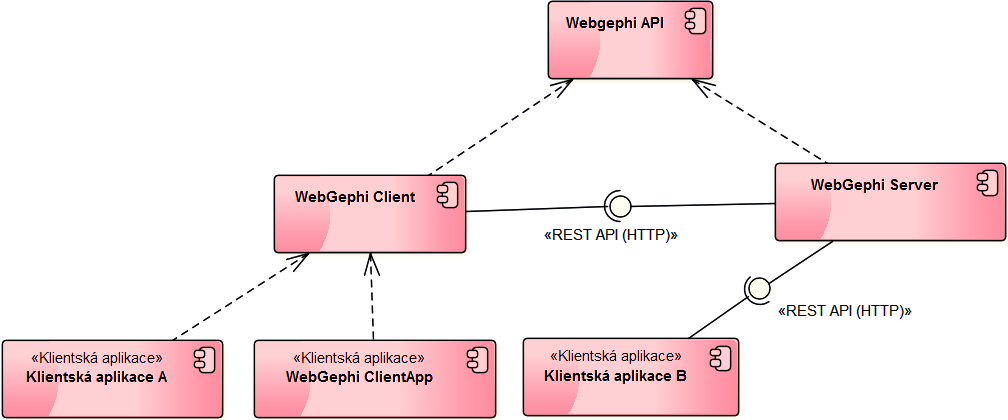
\includegraphics[width=1\textwidth]{images/diagram/modules}
 	\caption[Struktura WebGephi modulů]{Struktura WebGephi aplikací a jejich modulů}\label{fig:modules}
\end{figure}


\subsection{Server}
Serverová aplikace (dále jen \textit{Server} nebo \textit{WebGephi Server}) je základní aplikací, která realizuje samotné operace s grafy a řeší správu uživatelů.
\textit{WebGephi Server} poskutuje přístup ke své funkcionalitě pomocí REST rozhraní. Vytvoření této aplikace je hlavním cílem této práce.

\subsection{Klient (Java konektor)}
Přítup k \textit{Serveru} je umožněn pomocí REST webových služeb a autorizace pomocí OAuth protokolu\footnote{Basic autorizace je také možná, ale preferováno je použití OAuth protokolu.}.
Implementace OAuth klienta však není triviální. Proto bude pro potřeby klientských aplikací vytvořen \uv{konektor} k \textit{WebGephi Serveru} (dále jen \textit{Client} nebo \textit{WebGephi Client}).
Ten bude umožňovat jednoduché vytvoření autorizovaného připojení k \textit{Serveru} a poskytovat Java metody pro přístup ke zdrojům REST rozhraní.

\textit{WebGephi Client} bude standardní Java knihovnou, jeho použití tedy bude limitováno na klientské aplikace implementované v jazyku Java.

\subsection{Klientská aplikace}
Klientskou aplikací je míněna jakákoli aplikace využívající REST rozhraní \textit{Serveru}. A to buď přímo (například JavaScriptové aplikace), nebo pomocí knihovny \textit{WebGephi Client} (Java aplikace).
Součástí práce bude vytvoření ukázkové klientské aplikace (dále jen \textit{ClientApp} nebo \textit{WebGephi ClientApp}). Ta bude se \textit{Serverem} komunikovat pomocí knihovny \textit{Client}.
V podstatě se bude jednat o grafickou nadstavbu nad REST rozhranním serveru.

Na obr. \ref{fig:clientApp-proces} je znázorněn proces použití \textit{ClientApp}. Klientská aplikce nejdříve přesměruje uživatele na \textit{Server}, aby jí udělil oprávnění přistupovat k jeho účtu.
Po přihlášení deleguje veškeré operace s grafy na REST rozhraní serveru a pouze zobrazuje výsledky.

\begin{figure}\centering
 	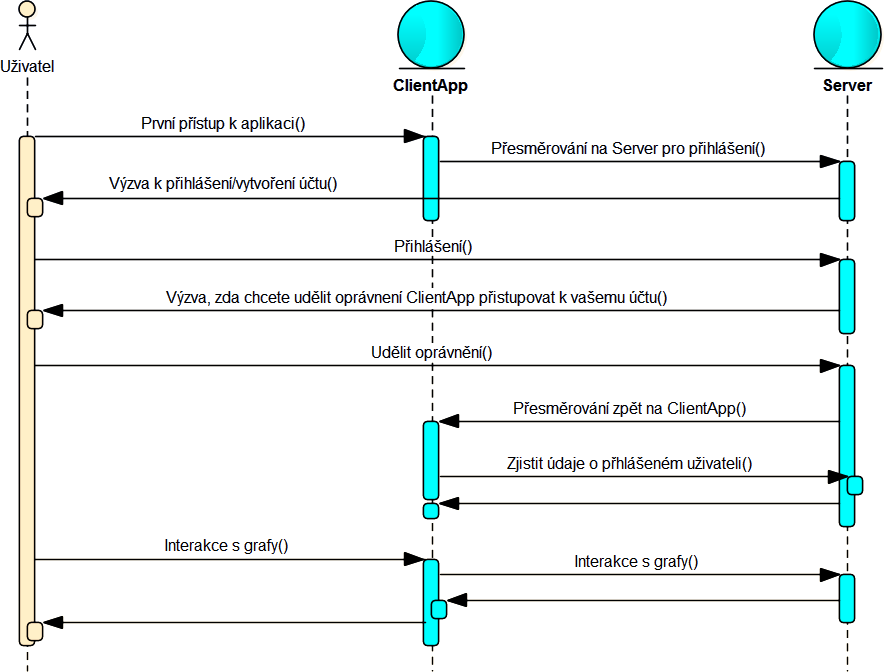
\includegraphics[width=1\textwidth]{images/diagram/clientApp-proces}
 	\caption[Proces používání \textit{ClientApp}]{Proces používání \textit{ClientApp}}\label{fig:clientApp-proces}
\end{figure}


\chapter{Realizace}
Na základě předchozích kapitol (analýzy a návrhu) byla implementována aplikace \textit{WebGephi} (\textit{Server}, \textit{Client} a všechny související moduly).
V této kapitole popíšeme způsob implementace, použité technologie a co vedlo k jejich výběru.

\section{Použité technologie}
V současné době se téměř žádné aplikace nestaví na zelené louce, jen s prostředky poskytovanými samotným jazykem. U webových aplikací 
toto platí stonásobně. Během vývoje se řeší stále stejné problémy, vytvoření webového GUI, práce s databází a management transakcí, serializace a deserializace 
objektů do XML, \ldots

Pro zjednodušení a urychlení vývoje, aby nebylo nutné stále znovu vynalézat kolo, vznikly kolekce knihoven řešící tyto problémy - \uv{frameworky}. Mnoho 
těchto frameworků bylo použito i při vývoji \textit{WebGephi}. 

\subsection{JavaEE\cite{javaEE}}
JavaEE\footnote{Java Platform, Enterprise Edition} není framework v právém slova smyslu. Jedná se o verzi jazyka javy 
rozšířenou o technologie vhodné pro vývoj tzv. \uv{Enterprise} aplikací - podnikové a webové aplikace, pro které je charakteristická potřeba 
integrace s jinými systémy. Aplikace pro platformu Java EE jsou vyvíjeny na základě API a dalších fragmentů definovaných v jednotlivých specifikacích.
Běhovým prostředím jsou tzv. aplikační servery, které jsou vyvíjeny různými společnostmi. Např. společnost Oracle vyvíjí aplikační server \textit{GlassFish}, který je
referenční implementací. Mezi další známe servery patří JBoss AS (nyní Wildfly), IBM WebSphere a WebLogic.
Vyvíjené aplikace by měli být mezi těmito servery libovolně přenostitelné. Mnoho z nich však obsahuje svá proprietární rozšíření, která mohou tuto přenositelnost narušit.

Součástí specifikace je např. technologie Java Server Faces (JSF), Java Persistence API (JPA), Enterprise Java Beans (EJB) a Contexts and Dependency Injection (CDI). 

Historickým konkurentem
JavaEE je proprietární open-source framework Spring\cite{spring}. Ten byl populární především v době JavaEE 1.4, kdy byla velmi těžkopádná a složitá na konfiguraci. Od té doby prošla JavaEE
velkým vývojem a převzala mnoho myšlenek právě od frameworku Spring. V dnešní době jsou tyto dvě platformy rovnocené a z velké části využívají i stejné frameworky.

Nejnovější verzí je JavaEE 7, která byla vydána v roce 2013. Tato verze také byla použita při vývoji aplikace \textit{WebGephi}. Před platformou Spring jsem jí dal přednost především kvůli svým
zkušenostem s touto technologií.

\subsection{Wildfly 8\cite{wildfly}}
Wildfly (dříve JBoss AS) je open-source aplikační server od společnosti JBoss. Osmá verze tohoto aplikačního serveru je plně kompatibilní s JavaEE 7.
Mezi jeho hlavní rysy patří rychlý start, malá spotřeba paměti a modularita.

Komerční verze tohoto serveru se nazývá JBoss EAP\footnote{Enterprise Application Platform}. Jedná se v zásadě o stejný server jako Wildfly, obsahuje 
však jen stabilní, ověřené verze modulů a zahrnuje také placenou podporu.

Tomuto serveru jsem dal přednost před jinými především kvůli svým dobrým zkušenostem s ním. Je využíván i v komerčním prostředí a jeho hlavním benefitem je rychlost
a přehledná konfigurace. Migrace na jiný aplikační server však není problém, je pouze třeba dát pozor na používání proprietárních deployment deskriptorů.

\subsection{JAX-RS\cite{jaxrs}}
JAX-RS je standardní JavaEE technologie pro deklarativní vývoj REST webových služeb. Pomocí anotací se označí metody, které mají být zveřejněny jako webové
služby (viz ukázka \ref{jaxrs-sample}). Aplikační server se pak postará o jejich zveřejnění. Tuto technologii používá \textit{WebGephi Server} pro
implementaci REST rozhraní.

\begin{lstlisting}[caption=Definice RESTful služby pro import grafu, label=jaxrs-sample, language=java]
@POST   
@Consumes(MediaType.TEXT_XML)
@Produces(MediaType.TEXT_XML)
public GraphXml addGraph(String document, @PathParam("user") String user, @QueryParam("name") String name, @QueryParam("format") String format) {
   ...
}
\end{lstlisting} 

JAX-RS je pouze specifikace, v současnosti existují dvě implementace: referenční Jersey od společnosti Oracle a RestEasy od společnosti JBoss. Aplikační server Wildfly přirozeně
obsahuje RestEasy implementaci.

JAX-RS používá technologii JAXB\footnote{Java Architecture for XML Binding\cite{jaxb}}. Ta je přímo součástí JDK a slouží k jednoduché deklarativní serializaci a deserializaci objektů do XML.
\textit{WebGephi} JAXB modelové objekty jsem vyčlenil do modulu \textit{WebGephi API}, aby mohly být znovupoužity v modulu \textit{WebGephi Client} (viz diagram \ref{fig:modules}).

Od verze 7 je součástí JavaEE platformy také standardizovaný REST klient. Ten je použit v modulu \textit{WebGephi Client}.

\subsection{Java Persistence API}
Objektový model aplikace založený na objektovém paradigma se příliž neslučuje se světem relačních databází. Pro jejich integraci
bylo vyvinuto mnoho frameworků. Nejrozšířenějším frameworkem v Java světě je JPA, v současnosti ve verzi 2.0.

Java Persistence API (JPA) je technologie pro práci s databází založená na objektovém přístupu. Java objekty jsou mapovány na databázové tabulky, případně 
vztahy mezi nimi. Programátor je tak odstíněn od databáze a místo s ní pracuje s tzv. Entity manažerem. Ten poskytuje metody pro ukládání (\texttt{persist(entity)}, \texttt{merge(entity)}), 
načítání (\texttt{find(class, id)}) a dotazování pomocí \texttt{Query} objektu.

Kromě absence nutnosti psát SQL dotazy mezi hlavní výhody JPA patří jednoduchá výměna implementace databáze a jednoduché kešování na úrovni Entity manažera.

JPA je pouze specifikace, nejrozšířenější implementace jsou Hibernate, OpenJPA a EclipseLink. Aplikace \textit{WebGephi Server} používá JPA (Hibernate) pro veškerou práci s databází.

\subsection{Enterprise Java Beans\cite{ejb}}
Enterprise Java Beans jsou serverové komponenty, jejichž životní cyklus je spravován kontejnerem. Používají se především pro implementaci bussiness logiky 
Enterprise aplikací. Poskutují služby jako je transakční zpracování, řízení souběžného přístupu, události pomocí JMS, jmenné a adresářové služby JNDI, interceptory.

Existují tři základní typy EJB: \texttt{Stateles}, \texttt{Stateful} a \texttt{Singleton}. Aplikace \textit{Gephi Server}  využívá EJB pro inicializaci 
po deploymentu (\texttt{Singleton}), jako DAO\footnote{Data Access Object} objekty a koncové body JAR-RS (\texttt{Stateles}). Využívá především schopností 
řízení souběžného přístupu, deklarativní správu transakcí a možnost navázání bussiness logiky po deploymentu aplikace. 

\subsection{CDI}
CDI\footnote{Contexts and Dependency Injection for Java EE\cite{cdi}} je součástí JavaEE od verze 6. Vzniklo na základě stížností, že koncept EJB je příliž těžkopádný a náročný na zdroje. Jedná se tedy o odlehčenou alternativu a doplněk k Enterprise Java Beans.
Poskytují např. možnost navázání interceptorů k metodám, možnost injektu závislostí, vlastní messaging systém a od verze JavaEE 7 také schopnost deklarativného řízení transakcí.

\textit{WebGephi Server} využívá CDI interceptorů pro ověřování autorizace uživatele. V aplikaci \textit{ClientApp} za využívá CDI messaging systém pro notifikaci grafických komponent pokud 
došlo k nějaké globální akci (např. pokud se změnil aktuální graf).

\subsection{GUI frameworky}
Standardní technologií pro tvorbu GUI v JavaEE je komponentový framework Java Server Faces (JSF). Ten je vhodný především pro formulářové aplikace, které jsou běžné
v podnikovém prostředí. Bohužel, jedná se o relativně starou technologii, do které byla např. podpora pro AJAX přidána až ve verzi 2.0. 
Není tedy příliš vhodný pro tvorbu moderních AJAXových aplikací, kde server slouží jen jako zdroj dat a prezentační logika je řízena přímo na klientovi (prohlížeči).

Proto jsem dal při implementaci \textit{WebGephi} přednost frameworkům založeným na Google Web Toolkit (GWT)\cite{gwt}\cite{gwt-in-action}.

\subsubsection{GWT}
GWT je framework od společnosti Google, umožňující jednoduchou tvorbu RIA\footnote{Rich Internet Application} aplikací v jazyku Java. 
Většina existujících technologií pro tvorbu RIA, jako je Flash, JavaFX nebo Silverlight, jsou nové programovací jazyky. 
Pro spuštění takovýchto aplikací je potřeba mít v prohlížeči nainstalovaný příslušný plugin.

GWT k problému přistupuje jinak. Všechny moderní prohlížeče mají nativní podporu skriptovacího jazyku JavaScript.
 Problémem JavaScriptu je, že původně byl konstruován jen pro drobné změny ve struktuře stránky. Je tedy velmi náročné udržovat 
 rozsáhlejší aplikaci napsanou v JavaScriptu. GWT řeší problém tím, že poskytuje překladač, který dokáže Java kód přeložit do JavaScriptu.

V principu jednoduchá myšlenka, ale s obrovskými dopady. Programátoři téměř vůbec nemusí znát JavaScript, píší celou aplikaci 
(klientskou i serverovou část) v Javě. To jim umožňuje používat všechny výhody Javy, jako jsou typovost, objektový přístup, dědičnost a také 
možnost testování kódu např. pomocí frameworku JUnit. Část kódu, která běží na klientovi, je při překladu přeložena do JavaScriptu
(optimalizovaného na rychlé zobrazení a malou velikost souborů - není nutné udržovat kód přehledný) a může být spuštěna ve webovém prohlížeči.
 
GWT je velmi mocný framework, zároveň však dost nízkoúrovňový. Proto vznikly další frameworky, které obsahují komplexnější logiku a využívají GWT překladač pro 
překlad do JavaScriptu. Příkladem těchto frameworků je Errai a Vaadin.

\subsubsection{Errai}
Framework Errai\cite{errai} si vzal za cíl přinést výhody JavaEE i do prohlížeče. To samozřemě není možné v plném rozsahu. Mezi jeho hlavní výhody patří
podpora injektu závislostí, mapování atributů kontrolerů do HTML šablon a podpora pro CDI messaging (i obousměrně mezi prohlížečem a serverem).

Tento framework jsem použil pro tvorbu grafického rozhraní aplikace \textit{WebGephi Server} pro správu uživatelů a klientských aplikací.
A to především z důvodu, že je paměťově velmi nenáročný - veškerá logika běží v prohlížeči v JavaScriptu a server slouží jen jako zdroj dat.

\subsubsection{Vaadin}\label{sec:vaadin}
Vaadin\cite{vaadin} je na rozdíl od frameworku Errai serverový framework. GUI komponenty jsou umístěny na serveru a jejich stav se zrcadlí 
v prohlížeči. Pokud např. uživatel klikne v prohlížeči na tlačítko, informace o akci se přenese na server v krátkém ajaxovém dotazu, kde se vyhodnotí navázaná akce
a poté se aktualizuje stav komponent v prohlížeči.

Tento model má výhody i nevýhody. Výhodou je možnost psát aplikace stejným způsobem jako desktopové aplikace, rychlý vývoj a možnost využití všech schopností JavaEE kontejneru.
Nevýhodou je větší paměťová náročnost, protože všechny komponenty jsou drženy v session na serveru. Po každé uživatelské operací je také potřeba komunikace se serverem, což vede k prodlevě mezi akcí 
a reakcí systému. Na druhou stranu jsou AJAXové dotazy velmi krátké, což paradoxně může vést k rychlejší odezvě, než při použití jiných technologií. V případě nutnosti Vaadin také umožňuje
vytvoření svých vlastních grafických komponent pomocí GWT.

Framework Vaadin jsem použil při implementaci aplikace \textit{WebGephi ClientApp} a to především z důvodu rychlého a jednoduchého vývoje.

\section{WebGephi Server}
\textit{WebGephi Server} se skládá z několika logických komponent. Jejich struktura a závislosti jsou znázorněny na diagramu \ref{fig:webgephi-server-impl}.

\begin{figure}\centering
 	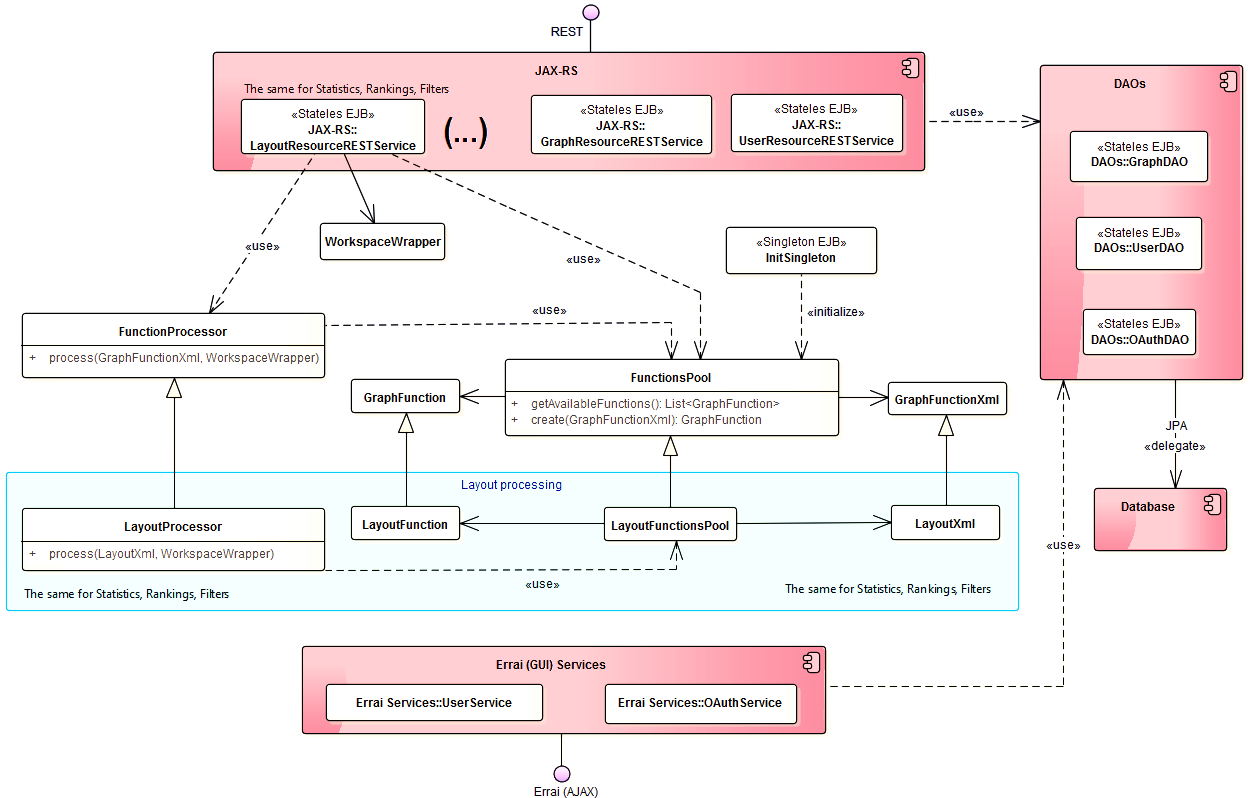
\includegraphics[width=1\textwidth]{images/diagram/webgephi-server-impl}
 	\caption[Struktura aplikace \textit{WebGephi Server}]{Struktura aplikace \textit{WebGephi Server}}.\label{fig:webgephi-server-impl}
\end{figure}

\subsection{DAOs}
\textit{WebGephi Server} využívá k přístupu technologii JPA. Přesto je její použití ještě obaleno použitím tzv. Data Access Objektů.
To umožňuje v budoucnu např. záměnu úložiště grafů za NoSQL databázi.

\subsection{Třídy pro zpracování grafových funkcí}
Tyto třídy jsou jádrem \textit{WebGephi} a obsahují hlavní bussiness logiku. Po deploymentu aplikace proběhne scan tříd a do \texttt{FunctionsPool}ů se uloží všechny dostupné 
grafové funkce. O aplikaci funkce na graf se starají implementace třídy \texttt{FunctionProcessor}. Ty z xml definice funkce (JAXB třídy) vytvoří její instanci a aplikují
ji na \textit{Gephi} workspace (\texttt{WorkspaceWrapper}).

Všechny tyto třídy (\texttt{FunctionsPool}, \texttt{FunctionProcessor}, \texttt{GraphFunction} a \texttt{FunctionXml}) mají svou vlastní implementaci pro každou kategorii funkcí (Layouts, Statistics, Rankings a Filters).
To v budoucnu umožňuje snadné rozšíření o další funkcionalitu, např. o \uv{Generátory}.

\subsection{REST rozhraní}
REST rozhraní je tvořeno JAX-RS třídami, které obsahují funkce pro obsluhu jednotlivých zdrojů. Využívají jak DAO komponenty, tak i třídy pro zpracování grafových funkcí.
Součástí aplikace \textit{WebGephi Server} je i dokumentace pro vývojáře popisující strukturu REST rozhraní a jednotlivých zdrojů. XML formát příchozích požadavků a odpovědí je navíc 
definován pomocí vlastního XSD schématu.

\subsection{Správa uživatelů a klientských aplikací}
Rozhraní pro správu uživatelů, OAuth autorizaci a správu klientských aplikací je implementováno pomocí frameworku Errai, který je rozšířením GWT.
Skládá se z klientské (package \texttt{cz\-.cokrtvac\-.webgephi\-.webgephiserver\-.gwt\-.client}) a serverové (package \texttt{cz\-.cokrtvac\-.webgephi\-.webgephiserver\-.gwt\-.server}) části.
Klientský kód je během buildu aplikace přeložen do html a JavaScriptu, běží ve webovém prohlížeči a vytváří grafické uživatelské rozhraní. Komunikuje se serverem za pomoci AJAXu a volá 
službu serverové části. Serverová část se stará o kontrolu autorizace a komunikuje s databází (DAO).

\begin{figure}\centering
 	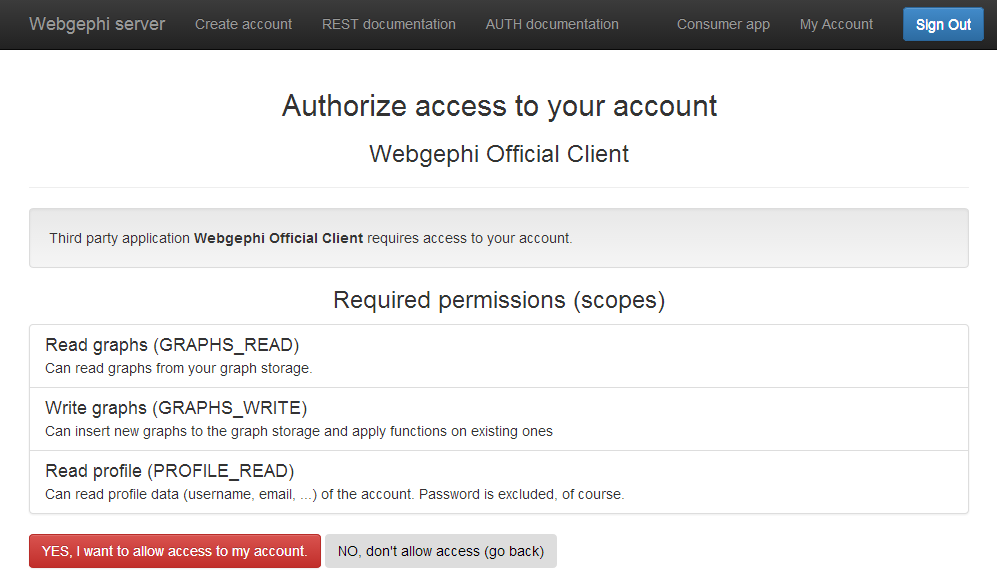
\includegraphics[width=0.8\textwidth]{images/prtsc/server-auth_request}
 	\caption[\textit{WebGephi Server} - Ukázka GUI (žádost o autorizaci aplikace)]{\textit{WebGephi Server} - Ukázka GUI (žádost o autorizaci aplikace)}.\label{fig:server-auth_request}
\end{figure}


\section{WebGephi Client}
\textit{Webgephi Client} je Java knihovna pro zjednodušení komunikace s REST rozhraním \textit{WebGephi Serveru}. Klientské aplikace 
implementované v jazyku Java mohou tuto knihovnu využít, aby nemusely implementovat své vlastní řešení pro OAuth autentizaci a volání RESTful služeb.

K autorizaci (získání OAuth request tokenu) slouží třída \texttt{WebgephiAuthen\-ticator}. Poté můžeme vytvořit samotný konektor - třidy implementující 
rozhraní \texttt{WebgephiClient}. Tyto třídy jsou struktutovány podobně jako In\-put/Out\-put streamy v JDK (viz class diagram \ref{fig:webgephi-client-impl}). Základní třída \texttt{Webgephi\-OAuthClient} umí pouze
volat HTTP metody (\texttt{GET, POST, PUT}) podepsané OAuth Request tokenem. Třída \texttt{WebgephiEntityClientImpl} umí již volat konkrétní zdroje \textit{WebGephi Server}, 
přičemž používá jednodušší \texttt{Webgephi\-Client} předaný v konstruktoru. Třída \texttt{Caching\-Webgephi\-Entity\-Client} umí navíc ještě kešovat neměné zdroje. Vytvoření kešovaného klienta 
je znázorněno v ukázce \ref{client-sample} 

\begin{figure}\centering
 	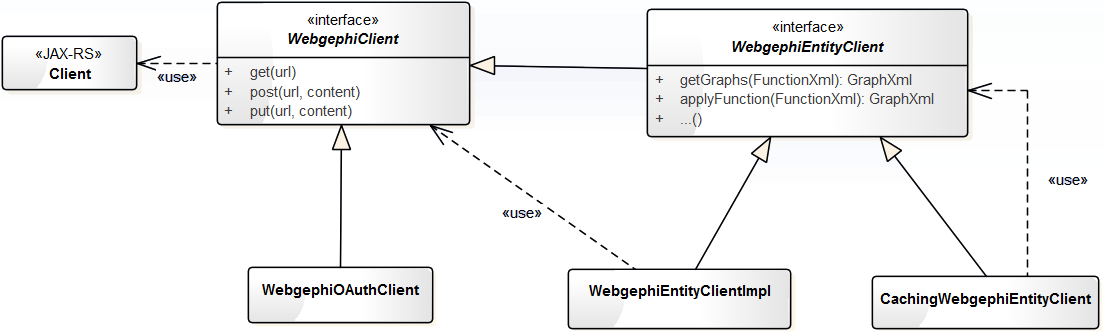
\includegraphics[width=1\textwidth]{images/diagram/webgephi-client-impl}
 	\caption[Struktura \textit{WebGephi} konektorů (klientů)]{Struktura \textit{WebGephi} konektorů (klientů)}.\label{fig:webgephi-client-impl}
\end{figure}

\begin{lstlisting}[caption=Vytvoření \texttt{CachingWebgephiEntityClient}, label=client-sample, language=java]
WebgephiEntityClient client = new CachingWebgephiEntityClient(new WebgephiEntityClientImpl(new WebgephiOAuthClient("https://webgephi.local:8443/rest/v1", accessToken)));
\end{lstlisting} 

\section{WebGephi ClientApp}
Aplikace \textit{ClientApp} slouží k demonstraci funkčnosti \textit{WebGephi Serveru}. Zároveň slouží jako ukázková aplikace pro vývojáře klientských aplikací. Jedná se 
o grafickou nadstavbu nad REST rozhraním, která umožňuje interakci se \textit{Serverem} téměř v plném rozsahu. Aplikace je implementována pomocí framworku 
pro tvorbu uživatelského rozhraní Vaadin (viz kapitola \ref{sec:vaadin}).

Uživatel se nejdříve musí přihlásit pomocí protokolu OAuth na \textit{Serveru} - je přesměrován na žádost o udělení přístupu ke jeho účtu. Po schválení žádosti je
přesměrován zpět a v grafické podobě je mu zobrazen obsah jeho grafového úložiště (obr. \ref{fig:clientapp-overview}). 

Výběrem grafu v pravé části obrazovky se zobrazí jeho detail ve středním panelu. Na aktuální graf je možno aplikovat libovolné grafové funkce - nabídka v levé části obrazovky.
Aplikace také umožňuje nahrání vlastního grafu v libovolném formátu. 

\begin{figure}\centering
 	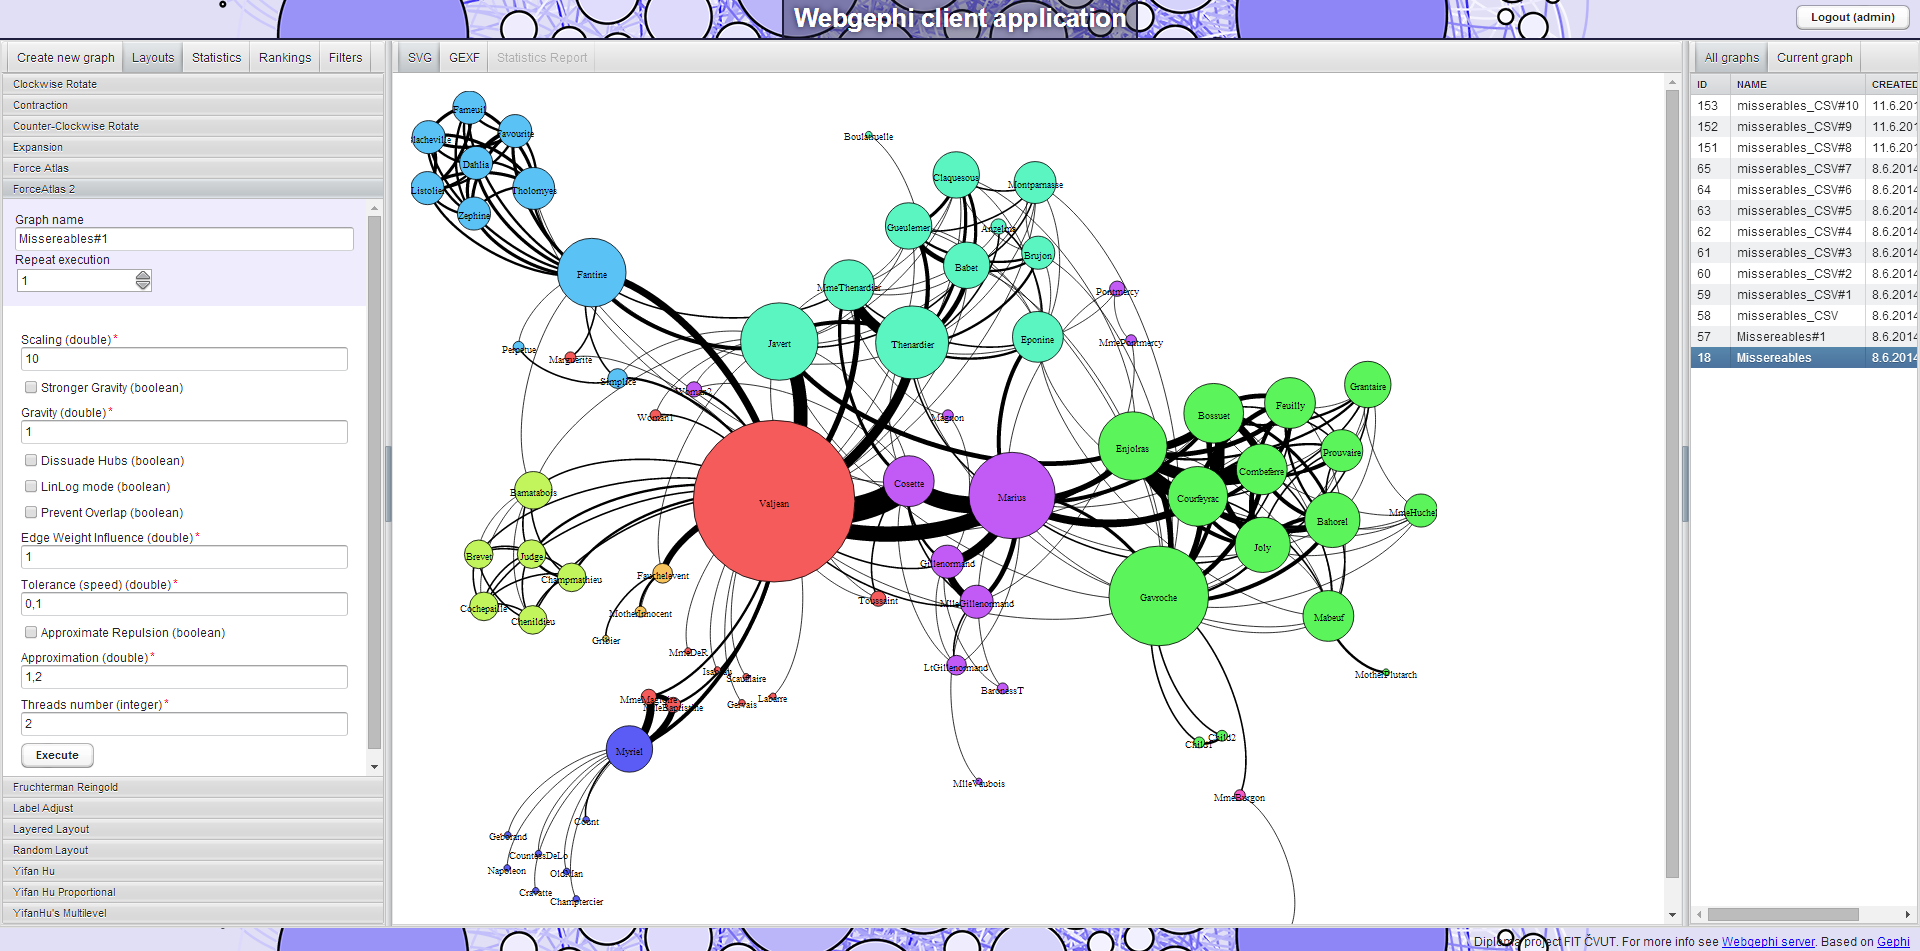
\includegraphics[width=1\textwidth]{images/prtsc/clientapp-overview}
 	\caption[Náhled aplikace \textit{WebGephi Client App}]{Náhled aplikace \textit{WebGephi Client App}}.\label{fig:clientapp-overview}
\end{figure}

\chapter{Testování}
Něco málo o testování

\section{Jednotkové testy}

\section{Integrační testy}
Testy REST rozhraní s použitím \textit{WebGephi Client}.

\section{Zátěžové testy}
JMeter

\begin{conclusion}
	Aplikace \textit{WebGephi} byla implementována v celém rozsahu zadání.
\end{conclusion}

\bibliographystyle{csn690}
\bibliography{mybibliographyfile}

\appendix
\chapter{Seznam použitých zkratek}
% \printglossaries
\begin{description}
	\item[GUI] Graphical user interface
	\item[XML] Extensible markup language
\end{description}

\chapter{Gephi}
\begin{figure}\centering
 	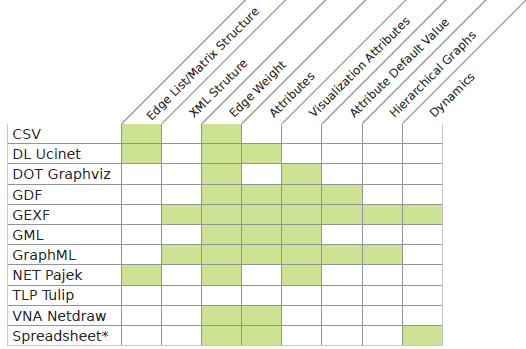
\includegraphics[width=1\textwidth]{images/gephi/graph-format-table-comparison}
 	\caption[Porovnání formátů vhodných pro ukládání grafů]{Porovnání formátů vhodných pro ukládání grafů. Převzato z \cite{gephi}}.\label{fig:gephi-formats-comparation}
\end{figure}

\chapter{Náhledy uživatelského rozhraní}
\section{WebGephi Server}
PrintScreens\ldots
\section{WebGephi Client Application}
PrintScreens\ldots

\chapter{Instalační příručka}

\chapter{Obsah přiloženého CD}

%upravte podle skutecnosti

\begin{figure}
	\dirtree{%
		.1 readme.txt\DTcomment{stručný popis obsahu CD}.
		.1 exe\DTcomment{adresář se spustitelnou formou implementace}.
		.1 src.
		.2 impl\DTcomment{zdrojové kódy implementace}.
		.2 thesis\DTcomment{zdrojová forma práce ve formátu \LaTeX{}}.
		.1 text\DTcomment{text práce}.
		.2 thesis.pdf\DTcomment{text práce ve formátu PDF}.
		.2 thesis.ps\DTcomment{text práce ve formátu PS}.
	}
\end{figure}

\end{document}
